
\documentclass[12pt,a4paper]{article}
\usepackage{composites2017}
% \usepackage{biblatex-trad} % for style unsrt

%%%%%%%%%%%%%%%%%%%%%%%%%%%%%%%%%%%%
% Header                           %
%%%%%%%%%%%%%%%%%%%%%%%%%%%%%%%%%%%%
%
% Compilation:
%
% - with pdfLaTeX:
%   pdflatex -> biber -> makeindex/create_glossaries.cmd -> pdflatex -> pdflatex
% - For compilation add switch -shell-escape in your LaTeX editor:
%   pdflatex --shell-escape -synctex=1 -interaction=nonstopmode %source --extra-mem-top=60000000
% - Compile at least 3 times for proper output
%
% In case of problems:
%
% - Increase Tex-Memory in batch with:
%   initexmf --edit-config-file pdflatex
%   add: main_memory=8000000
%   initexmf --dump=pdflatex
%
% Revisions: 2017-04-10 Martin Rädel <martin.raedel@dlr.de>
%                       Initial draft
%
% Contact:   Martin Rädel,  martin.raedel@dlr.de
%            DLR Composite Structures and Adaptive Systems
%
%                                 __/|__
%                                /_/_/_/  
%            www.dlr.de/fa/en      |/ DLR
%
%%%%%%%%%%%%%%%%%%%%%%%%%%%%%%%%%%%%
% Preamble                         %
%%%%%%%%%%%%%%%%%%%%%%%%%%%%%%%%%%%%

% ---------------------------
% Path to common
% ---------------------------

\newcommand{\peridoccommonpath}{../../../../Doc/PeriDoX_Common}
\newcommand{\peridocliteraturepath}{../../../../Literature}
\newcommand{\materialpath}{../../Material}

% ---------------------------
% Local packages
% ---------------------------

\usepackage[
  style=numeric-comp,
  sorting=none,
  url=false,
  isbn=false
]{biblatex}
\usepackage{booktabs}
\usepackage{caption}
\usepackage{enumitem}
\usepackage{filecontents}
\usepackage{multirow}
% \usepackage{placeins} % for \FloatBarrier
\usepackage{siunitx}
\sisetup{%
  exponent-product = \cdot,%
  output-product = \cdot,%
  separate-uncertainty=true,% uncertainty is separated with a "plus-minus" symbol
}
\usepackage{subcaption}
\usepackage{tabularx}

% General preamble
% %%%%%%%%%%%%%%%%%%%%%%%%%%%%%%%%%%%%
% Header                           %
%%%%%%%%%%%%%%%%%%%%%%%%%%%%%%%%%%%%
% 
% This file handles all things with general packages
% 
% Revisions: 2017-04-10 Martin Raedel <martin.raedel@dlr.de>
%                       Initial draft
%               
% Contact:   Martin Raedel,  martin.raedel@dlr.de
%            DLR Composite Structures and Adaptive Systems
%          
%                                 __/|__
%                                /_/_/_/  
%            www.dlr.de/fa/en      |/ DLR
% 
%%%%%%%%%%%%%%%%%%%%%%%%%%%%%%%%%%%%
% Content                          %
%%%%%%%%%%%%%%%%%%%%%%%%%%%%%%%%%%%%

% ---------------------------
% Packages
% ---------------------------

% Every package with the exception of
% - RMLaTeX-packages
% - Hyperref
% - Every package that has to be placed after hyperref -> Pref_Packages_Hyperref.tex
\usepackage[latin1]{inputenx}
\usepackage[T1]{fontenc}
\usepackage{amsmath}
\usepackage{amssymb}
\usepackage{amsthm}
\usepackage[page,titletoc]{appendix}
\usepackage{array}
% babel package is loaded seperately. Allows reuse for projects with various languages
% biblatex package is loaded in Pref_BibLaTeX_XYZ.tex from PeriDoc_Common
\usepackage{booktabs}
\usepackage{caption}
\usepackage{calc}
\usepackage{color}
\usepackage{coseoul}
\usepackage{csquotes}
\usepackage{enumitem}
\usepackage{esvect}
\usepackage{etoolbox}
\usepackage{filecontents}
% http://tex.stackexchange.com/a/312910/44634 for fixing clash between filecontents and morewrites
\newwrite\fcwrite
\makeatletter
\let\zzzz\filec@ntents
\def\filec@ntents{\def\chardef##1\write{\let\reserved@c\fcwrite}\zzzz}
\makeatother
% Mute "Overwriting file" warning for filecontents package
\usepackage{ifthen}
\usepackage{ltxtable}
\usepackage{marginnote}
\usepackage{marvosym}                            % Symbols: \Faxmachine, \Mundus, \Letter
\usepackage{mathtools}
\usepackage{media9}
\usepackage{morewrites}                          % http://tex.stackexchange.com/q/289734
\usepackage{multicol}
\usepackage{multirow}
%\usepackage{nomencl}
\usepackage{pifont}
\usepackage{placeins}
\usepackage{subcaption}
\usepackage{tabto}
\usepackage{tabu}
\usepackage{tabularx}
\usepackage[most]{tcolorbox}
\usepackage{textcomp}

\makeatletter
\@ifundefined{KOMAClassName}
  {% true -> no KOMA class
    \@ifclassloaded{amsart}{
      % Do nothing! Amsart does not play with titlesec package
    }{
      \usepackage{titlesec}    
    }
  }
  {% false -> KOMA class
  }
\makeatother

\usepackage[figure,table,lstlisting]{totalcount}
\usepackage{upquote}
\usepackage{wasysym}                            % Symbols \& Smileys :)
\usepackage{wrapfig}
\usepackage{xparse}

\usepackage{hyphenat}
% %%%%%%%%%%%%%%%%%%%%%%%%%%%%%%%%%%%%
% Header                           %
%%%%%%%%%%%%%%%%%%%%%%%%%%%%%%%%%%%%
% 
% This file handles all things considering the hyperref package
%
% Requirements:
%
% - use of either Pref_Language_English.tex or Pref_Language_German.tex before this file
% 
% Revisions: 2017-04-10 Martin Raedel <martin.raedel@dlr.de>
%                       Initial draft
%               
% Contact:   Martin Raedel,  martin.raedel@dlr.de
%            DLR Composite Structures and Adaptive Systems
%          
%                                 __/|__
%                                /_/_/_/  
%            www.dlr.de/fa/en      |/ DLR
% 
%%%%%%%%%%%%%%%%%%%%%%%%%%%%%%%%%%%%
% Content                          %
%%%%%%%%%%%%%%%%%%%%%%%%%%%%%%%%%%%%

% ---------------------------
% Load package
% ---------------------------

% https://tex.stackexchange.com/questions/17218/make-hyperref-take-pdfinfo-from-title-and-author
\makeatletter
\@ifpackageloaded{hyperref}{}{
  \usepackage[%
    % These options must be set at the time of \usepackage and can not be set using \hypersetup
    bookmarks = true,
    pdfusetitle,%
  ]{hyperref}
}
\makeatother

% ---------------------------
% Package options
% ---------------------------

\makeatletter%
  \@ifclassloaded{elsarticle}{}{% elsarticle works with natbib instead of BibLaTeX
    \hypersetup{%
      colorlinks = true,%
      linkcolor  = black,%
      citecolor  = black,%
      urlcolor   = blue,%
      pdfstartview = Fit,%
      pdfmenubar = true,%
      pdftoolbar = true,%
      %
      bookmarksopen = false,
      %bookmarksopenlevel = 1,
    }
  }
\makeatother

% ---------------------------
% Renewcommand hyperref autorefnames
% ---------------------------

%cross references to equations with parenthesis
%\newcommand{\RefEq}[1]{\equationautorefname~\eqref{#1}}

%cross references to figures
%\newcommand{\RefFig}[1]{\figureautorefname~\ref{#1}}

%cross references to tables
%\newcommand{\RefTab}[1]{\tableautorefname~\ref{#1}}

% http://tex.stackexchange.com/questions/36575/autorefs-inserted-text-has-not-the-correct-case
\iflanguage{english}{
  \AtBeginDocument{
    \renewcommand*{\equationautorefname}{Equation}
    \renewcommand*{\figureautorefname}{Figure}
    \renewcommand*{\tableautorefname}{Table}
  }
}

\iflanguage{ngerman}{
  \AtBeginDocument{
    \renewcommand*{\equationautorefname}{Gleichung}
    \renewcommand*{\figureautorefname}{Abbildung}
    \renewcommand*{\tableautorefname}{Tabelle}
  }
}

% ---------------------------
% Packages after Hyperref
% ---------------------------

\usepackage{attachfile}
%%%%%%%%%%%%%%%%%%%%%%%%%%%%%%%%%%%%
% Header                           %
%%%%%%%%%%%%%%%%%%%%%%%%%%%%%%%%%%%%
% 
% This file handles all things considering the siunitx package
%
% Revisions: 2016-03-06 Martin Raedel <martin.raedel@dlr.de>
%                       Initial draft
%               
% Contact:   Martin Raedel,  martin.raedel@dlr.de
%            DLR Composite Structures and Adaptive Systems
%          
%                                 __/|__
%                                /_/_/_/  
%            www.dlr.de/fa/en      |/ DLR
% 
%%%%%%%%%%%%%%%%%%%%%%%%%%%%%%%%%%%%
% Content                          %
%%%%%%%%%%%%%%%%%%%%%%%%%%%%%%%%%%%%

%-----------------------------------
% Load package
%-----------------------------------

\usepackage{siunitx}

%-----------------------------------
% Setup
%-----------------------------------

\sisetup{%
  exponent-product = \cdot,%
  output-product = \cdot,%
  binary-units=true,%
}

%-----------------------------------
% New units
%-----------------------------------

% Length
\DeclareSIUnit\foot{ft}
\DeclareSIUnit\inch{in}

% Temperature
\DeclareSIUnit\degreeFahrenheit{^{\circ}F}
\DeclareSIUnit\degreeRankine{^{\circ}R}

% Force
\DeclareSIUnit\dyn{dyn}
\DeclareSIUnit\poundforce{lbf}

% Pressure
\DeclareSIUnit\barye{Ba}
\DeclareSIUnit\psi{psi}

% Density
\DeclareSIUnit\slug{slug}

% Energy
\DeclareSIUnit\erg{erg}

% Promille
\DeclareSIUnit[number-unit-product = \,]{\promille}{\textperthousand}
%%%%%%%%%%%%%%%%%%%%%%%%%%%%%%%%%%%%
% Header                           %
%%%%%%%%%%%%%%%%%%%%%%%%%%%%%%%%%%%%
% 
% This file handles all things considering the TikZ package
%
% Revisions: 2016-03-06 Martin Raedel <martin.raedel@dlr.de>
%                       Initial draft
%               
% Contact:   Martin Raedel,  martin.raedel@dlr.de
%            DLR Composite Structures and Adaptive Systems
%          
%                                 __/|__
%                                /_/_/_/  
%            www.dlr.de/fa/en      |/ DLR
% 
%%%%%%%%%%%%%%%%%%%%%%%%%%%%%%%%%%%%
% Content                          %
%%%%%%%%%%%%%%%%%%%%%%%%%%%%%%%%%%%%

% ---------------------------
% Load package
% ---------------------------

\makeatletter
\@ifpackageloaded{tikz}{
  %\usetikzlibrary{angles}
  \usetikzlibrary{arrows.meta}
  \usetikzlibrary{backgrounds}
  \usetikzlibrary{calc}
  \usetikzlibrary{decorations.markings}
  \usetikzlibrary{decorations.text}
  \usetikzlibrary{fit}
  % \usetikzlibrary{fpu}
  \usetikzlibrary{intersections}
  \usetikzlibrary{tikzmark}
  \usetikzlibrary{trees}
  \usetikzlibrary{matrix}
  \usetikzlibrary{patterns}
  \usetikzlibrary{positioning}
  \usetikzlibrary{shadows}
  % \usetikzlibrary{shapes}
  \usetikzlibrary{shapes.misc}
  \usetikzlibrary{spy}
}{
  \usepackage{tikz}
  %\usetikzlibrary{angles}
  \usetikzlibrary{arrows.meta}
  \usetikzlibrary{backgrounds}
  \usetikzlibrary{calc}
  \usetikzlibrary{decorations.markings}
  \usetikzlibrary{decorations.text}
  \usetikzlibrary{fit}
  % \usetikzlibrary{fpu}
  \usetikzlibrary{intersections}
  \usetikzlibrary{tikzmark}
  \usetikzlibrary{trees}
  \usetikzlibrary{matrix}
  \usetikzlibrary{patterns}
  \usetikzlibrary{positioning}
  \usetikzlibrary{shadows}
  % \usetikzlibrary{shapes}
  \usetikzlibrary{shapes.misc}
  \usetikzlibrary{spy}
}
\makeatother

% ---------------------------
% Pgfmath
% ---------------------------

\makeatletter
% Stuff for calc compatiability.
\let\real=\pgfmath@calc@real
\let\minof=\pgfmath@calc@minof
\let\maxof=\pgfmath@calc@maxof
\let\ratio=\pgfmath@calc@ratio
\let\widthof=\pgfmath@calc@widthof
\let\heightof=\pgfmath@calc@heightof
\let\depthof=\pgfmath@calc@depthof
\makeatother

% ---------------------------
% Tikzsets
% ---------------------------

% Default arrow tip
\tikzset{
  defarrow/.style={                           % Define arrow style
    >=Stealth,                                % >=latex
  }
}

\tikzset{
  every picture/.style=semithick              % Adjust default line width
}

% Help grid for external images
% Call inside scope with: \pic{myimagegrid};
\tikzset{%
  myimagegrid/.pic={%
   \draw[help lines,xstep=.1,ystep=.1] (0,0) grid (1,1);
   \foreach \x in {0,1,...,9} {\node [anchor=north] at (\x/10,0) {0.\x};}
   \foreach \y in {0,1,...,9} {\node [anchor=east]  at (0,\y/10) {0.\y};}
  }%
}

% Equal space decoration markers along addplot path
% http://tex.stackexchange.com/a/232010/44634
\makeatletter
\tikzset{
  nomorepostactions/.code={\let\tikz@postactions=\pgfutil@empty},
  mymark/.style 2 args={decoration={markings,
    mark= between positions 0 and 1 step (1/11)*\pgfdecoratedpathlength with{%
        \tikzset{#2,every mark}\tikz@options
        \pgfuseplotmark{#1}%
      },  
    },
    postaction={decorate},
    /pgfplots/legend image post style={
      mark=#1,
      #2,
      every path/.append style={nomorepostactions}
    },
  },
}
\makeatother

% Markup style for rectangles on external figures
% Needs Pref_Color.tex for mymarkupcolor
\tikzset{%
  myrectangularmarkup/.style={%
   inner sep=0pt,% necessary for correct positioning of corners
   draw=mymarkupcolor,%
   thick,%
  }%
}

\tikzset{%
  mymarkuptext/.style={%
   text=mymarkupcolor,%
  }%
}

% A croos for markings in plots
% https://tex.stackexchange.com/a/124064
\tikzset{cross/.style={cross out, draw, 
         minimum size=2*(#1-\pgflinewidth), 
         inner sep=0pt, outer sep=0pt}}

% ---------------------------
% Pgfkeys
% ---------------------------

% From the pgf manual 2.10csv page 694:
% 
%     It should be noted that all calculations must not exceed �16383.99999 at any point, because the underlying computations rely on TeX dimensions. This means that many of the underlying computations are necessarily approximate and that in addition, are not very fast. TeX is, after all, a typesetting language and not ideally suited to relatively advanced mathematical operations. However, it is possible to change the computations as described in Section 76.
% 
% From the TeX Book page 114:
% 
%     16383.99998pt (TeX's largest dimen)
% 
% In Notes On Programming in TeX Chirstian Feuersaenger pointed out
% 
%     The \dimen registers perform their arithmetic's internally with 32 bit scaled integers, so called scaled point with unit sp. It holds 1pt = 65536sp = 216sp. One of the 32 bits is used as sign. The total number range in pt is [-(2^30-1)/2^16,(2^30-1)/2^16 ]=[-16383.9998, +16383.9998]1.
% 
%     1 Please note that this does not cover the complete range of a 32 bit integer, I do not know why
% \pgfkeys{/pgf/fpu=true}                       % Allow pgf to plot values larger than 16383.9998
% \tikzset{fpu}                                   % Allow pgf to plot values larger than 16383.9998

\pgfkeys{/tikz/savenumber/.code 2 args={\global\edef#1{#2}}}

% ---------------------------
% tikzsets
% ---------------------------

%~~~~~ WaveChart Style ~~~~~~~~~~

\tikzset{
  wavespy style/.style={
    spy scope={%
      wavespyscope style,%
    },
    connect spies/.style={
      wavespyconnect style,%
    },
  }
}

\tikzset{
  wavespyscope style/.style={
    magnification=4,
    connect spies,                            % Connect orig. & detail
    width=2.0cm,                              % Spy width
    height=1.0cm,                             % Spy height
    every spy on node/.style={                % Source
      rectangle,                              % Form
      rounded corners,                        % Edge shape
      dashed,                                 % Dashed line
      draw=gray,                              % Line color
      thick,                                  % Line style for spy
    },
    every spy in node/.style={                % Spy
      rectangle,                              % Form
      rounded corners,                        % Edge shape
      dashed,                                 % Dashed line
      draw=gray,                              % Line color
      thick,                                  % Line style for spy
    },
  },
}

\tikzset{
  wavespyconnect style/.style={
    spy connection path={
      \draw[%
        thick,
        dashed,
        gray
      ] (tikzspyonnode) -- (tikzspyinnode); % In-On-Connection
    },
  },
}
%%%%%%%%%%%%%%%%%%%%%%%%%%%%%%%%%%%%
% Header                           %
%%%%%%%%%%%%%%%%%%%%%%%%%%%%%%%%%%%%
% 
% This file handles all things considering the pgfplots package
% 
% Revisions: 2017-04-10 Martin Raedel <martin.raedel@dlr.de>
%                       Initial draft
%               
% Contact:   Martin Raedel,  martin.raedel@dlr.de
%            DLR Composite Structures and Adaptive Systems
%          
%                                 __/|__
%                                /_/_/_/  
%            www.dlr.de/fa/en      |/ DLR
% 
%%%%%%%%%%%%%%%%%%%%%%%%%%%%%%%%%%%%
% Content                          %
%%%%%%%%%%%%%%%%%%%%%%%%%%%%%%%%%%%%

% ---------------------------
% Load package
% ---------------------------

% Pgfplots
\makeatletter
\@ifpackageloaded{pgfplots}{
  \usepgfplotslibrary{fillbetween}
  \usepgfplotslibrary{groupplots}
  \usepgfplotslibrary{patchplots}
}{
  \usepackage{pgfplots}
  \usepgfplotslibrary{fillbetween}
  \usepgfplotslibrary{groupplots}
  \usepgfplotslibrary{patchplots}
}
\makeatother

% Pgfplotstable
\makeatletter
\@ifpackageloaded{pgfplotstable}{}{
  \usepackage{pgfplotstable}
}
\makeatother


% Temporary fix for pgfplots & forest problems reported in September 2016
% here: http://tex.stackexchange.com/questions/328972/presence-of-pgfplots-package-breaks-forest-environment-w-folder-option-en
% \makeatletter
% \let\pgfmathModX=\pgfmathMod@
% \usepackage{pgfplots}%
% \let\pgfmathMod@=\pgfmathModX
% \makeatother

% ---------------------------
% Pgf version
% ---------------------------

\pgfplotsset{compat=1.14}

% ---------------------------
% colormaps
% ---------------------------

\pgfplotsset{
  colormap={abaqusblueredcolormap}{
    rgb255( 0cm)=(  0,  0,255);
    rgb255( 1cm)=(  0, 93,255);
    rgb255( 2cm)=(  0,185,255);
    rgb255( 3cm)=(  0,255,232);
    rgb255( 4cm)=(  0,255,139);
    rgb255( 5cm)=(  0,255,139);
    rgb255( 6cm)=(  0,255, 46);
    rgb255( 7cm)=( 46,255,  0);
    rgb255( 8cm)=(139,255,  0);
    rgb255( 9cm)=(232,255,  0);
    rgb255(10cm)=(255,185,  0);
    rgb255(11cm)=(255, 93,  0);
    rgb255(12cm)=(255,  0,  0);
  }
}

\pgfplotsset{
  colormap={paraviewblueredcolormap}{
    rgb255( 0cm)=(  0,  0,255);
    rgb255( 1cm)=(  0, 93,255);
    rgb255( 2cm)=(  0,185,255);
    rgb255( 3cm)=(  0,255,232);
    rgb255( 4cm)=(  0,255,139);
    rgb255( 5cm)=(  0,255,139);
    rgb255( 6cm)=(  0,255, 46);
    rgb255( 7cm)=( 46,255,  0);
    rgb255( 8cm)=(139,255,  0);
    rgb255( 9cm)=(232,255,  0);
    rgb255(10cm)=(255,185,  0);
    rgb255(11cm)=(255, 93,  0);
    rgb255(12cm)=(255,  0,  0);
  }
}

\pgfplotsset{
  colormap={whiteblack}{color(0cm)=(white);color(1cm)=(black)}
}

% ---------------------------
% pgfplotsset
% ---------------------------

%~~~~~ Number format ~~~~~~~~

% call with e.g.: y tick label style={numberformatfixed={3}}
\pgfplotsset{
    numberformatfixed/.style 2 args={
      /pgf/number format/fixed,
      /pgf/number format/fixed zerofill,% Allow trailing zeros
      /pgf/number format/precision=#1,   % Nr of decimal digits
    },
    numberformatfixed/.default={2}
}

%~~~~~ Colorbar ~~~~~~~~~~~~~

\pgfplotsset{
  basecolorbaraxis style/.style={
    hide axis,
    scale only axis,
    colormap/bluered,                         % Colormap preset
    colorbar sampled,                         % Steps in colorbar
  }
}

\pgfplotsset{
  damageaxis style/.style={
    basecolorbaraxis style,
    point meta min=0.0,                       % Minimum value colorbar
    point meta max=1.0,                       % Maximum value colorbar
  }
}

\pgfplotsset{
  damagefigureaxis style/.style={
    %basecolorbaraxis style,
    %point meta min=0.0,                       % Minimum value colorbar
    %point meta max=1.0,                       % Maximum value colorbar
    damageaxis style,
    enlargelimits=false,                      % Do not add margins
    axis equal image,                         % Keep aspect ratio
  }
}

\pgfplotsset{
  mybarundertensionaxis style/.style={
    hide axis,
    scale only axis,
    %anchor=east,
    anchor=west,
    height=0.125\textheight,
    %xshift=0.25cm,
    xshift=-1.0cm,
    colormap/bluered, % Colormap preset
    colorbar sampled, % Steps in colorbar
    colorbar right, % Activate colorbar
  }
}

\pgfplotsset{
  damagecolorbar style/.style={
    separate axis lines,
    samples=256,                              % Number of steps+1
  }
}

\pgfplotsset{
  abaqusdiscrete12colorbar style/.style={
    separate axis lines,
    samples=13,                               % Number of steps+1
  }
}

\pgfplotsset{
  abaqusdiscrete256colorbar style/.style={
    separate axis lines,
    samples=256,                              % Number of steps+1
  }
}

\pgfplotsset{
  ansysdiscrete9colorbar style/.style={
    separate axis lines,
    samples=10,                               % Number of steps+1
  }
}

\pgfplotsset{
  paraviewdiscrete256colorbar style/.style={
    separate axis lines,
    samples=256,                              % Number of steps+1
  }
}

%~~~~~ Chart Style ~~~~~~~~~~

\pgfplotsset{
  chart style/.style={
    width=0.7\linewidth,
    height=0.3\textheight,
    axis x line=middle,                       % Middle x-axis
    axis y line=left,
    enlarge x limits={auto,upper},            % Add this at positive x
    enlarge y limits,                         % Add this at y
    x label style={                           % xlabel style
      at={(axis description cs:0.5,-0.025)},  % Position
      anchor=north                            % Anchor
    },
    y label style={                           % ylabel style
      anchor=south                            % Anchor
    },
    x tick label style={
      /pgf/number format/fixed,
      /pgf/number format/precision=5,         % Nr of decimal digits
    },
    y tick label style={
      /pgf/number format/fixed,
      /pgf/number format/fixed zerofill,      % Allow trailing zeros
      /pgf/number format/precision=1,         % Nr of decimal digits
    },
    scaled ticks=false,
    legend columns=1,                         % Nr of colums in legend
    legend style={
      draw=none,                              % No border
      fill=none,                              % No fill color
      at={(1.025,0.5)},                       % Position
      anchor=west,                            % Anchor
      /tikz/row 2/.style={
        row sep=5pt,
      }
    }
  }
}

\pgfplotsset{
  xaxis style/.style={
    each nth point=1,
    restrict expr to domain={rawx}{0:5},      % restrict x-axis values
  }
}

%~~~~~ WaveChart Style ~~~~~~~~~~

\pgfplotsset{
  wavechart style/.style={
    chart style,
    xlabel={Time [ms]},
    ylabel={Displacement [mm]},
    ylabel near ticks,
    xticklabel={%
      \pgfkeys{/pgf/fpu=true}%               % Allow numbers > 16383.99
      \pgfmathparse{\tick*1000}%             % Scale s to ms
      \pgfkeys{/pgf/fpu=false}%              % Switch of fpu
      $\pgfmathprintnumber[
        fixed,                               % Number format
        precision=1,                         % Nr of decimal digits
      ]{\pgfmathresult}$%
    },
    yticklabel={%
      \pgfkeys{/pgf/fpu=true}%               % Allow numbers > 16383.99
      \pgfmathparse{\tick*1000}%             % Scale m to mm
      \pgfkeys{/pgf/fpu=false}%              % Switch of fpu
      $\pgfmathprintnumber[
        fixed,                               % Number format
        precision=1,                         % Nr of decimal digits
      ]{\pgfmathresult}$%
    },
  }
}

\pgfplotsset{
  wavexaxis style/.style={
    each nth point=1,
    restrict expr to domain={rawx}{0:0.005},   % restrict x-axis values [ms]
  }
}

%~~~~~ Tension chart ~~~~~~~~~

\pgfplotsset{
  tensionchart style/.style={
    chart style,
    enlarge y limits={auto,upper},           % Add this at positive y
    xlabel={Time [s]},
    ylabel={Displacement [mm]},
    xlabel near ticks,
    ylabel near ticks,
    yticklabel={%
      \pgfkeys{/pgf/fpu=true}%               % Allow numbers > 16383.99
      \pgfmathparse{\tick*1000}%             % Scale m to mm
      \pgfkeys{/pgf/fpu=false}%              % Switch of fpu
      $\pgfmathprintnumber[
        fixed,                               % Number format
        precision=1,                         % Nr of decimal digits
      ]{\pgfmathresult}$%
    },
  }
}

\pgfplotsset{
  tensionchart2 style/.style={
    tensionchart style,
    xlabel={Position bar in $x$-direction [m]},
    ylabel={Displacement [mm]},
  }
}

\pgfplotsset{
  dispxaxis style/.style={
    each nth point=1,
  }
}

%~~~~~ Energy chart ~~~~~~~~~

\pgfplotsset{
  energychart style/.style={
    chart style,
    xlabel={Time [ms]},
    ylabel={Energy [J]},
    xlabel near ticks,
    ylabel near ticks,
    enlarge y limits={auto,upper},            % Add this at positive y
    %x tick label style={
    %  /pgf/number format/fixed,
    %  /pgf/number format/precision=5,         % Nr of decimal digits
    %},
    y tick label style={
      /pgf/number format/fixed,
      %/pgf/number format/fixed zerofill,      % Allow trailing zeros
      /pgf/number format/precision=0,         % Nr of decimal digits
    },
    legend cell align=left,
    cycle list name=color list,               % colors !!! use addplot+ to cycle through colors !!!
    scaled x ticks=false,
    xticklabel={%
      \pgfkeys{/pgf/fpu=true}%               % Allow numbers > 16383.99
      \pgfmathparse{\tick*1000}%             % Scale s to ms
      \pgfkeys{/pgf/fpu=false}%              % Switch of fpu
      $\pgfmathprintnumber[
        fixed,                               % Number format
        precision=1,                         % Nr of decimal digits
      ]{\pgfmathresult}$%
    },
  }
}

\pgfplotsset{
  advenergychart style/.style={
    energychart style,
    scaled y ticks=false,
    yticklabel={%
      \pgfkeys{/pgf/fpu=true}%               % Allow numbers > 16383.99
      \pgfmathparse{\tick/1000}%             % Scale mJ to J
      \pgfkeys{/pgf/fpu=false}%              % Switch of fpu
      $\pgfmathprintnumber[
        fixed,                               % Number format
        precision=0,                         % Nr of decimal digits
      ]{\pgfmathresult}$%
    }
  }
}

%~~~~~ Displacement chart ~~~

\pgfplotsset{
  displchart style/.style={
    chart style,
    xlabel={Time [ms]},
    ylabel={Displacement [mm]},
    xlabel near ticks,
    ylabel near ticks,
    enlarge y limits={auto,upper},            % Add this at positive y
    %x tick label style={
    %  /pgf/number format/fixed,
    %  /pgf/number format/precision=5,         % Nr of decimal digits
    %},
    y tick label style={
      /pgf/number format/fixed,
      %/pgf/number format/fixed zerofill,      % Allow trailing zeros
      /pgf/number format/precision=1,         % Nr of decimal digits
    },
    legend cell align=left,
    scaled x ticks=false,
    xticklabel={%
      \pgfkeys{/pgf/fpu=true}%               % Allow numbers > 16383.99
      \pgfmathparse{\tick*1000}%             % Scale s to ms
      \pgfkeys{/pgf/fpu=false}%              % Switch of fpu
      $\pgfmathprintnumber[
        fixed,                               % Number format
        precision=1,                         % Nr of decimal digits
      ]{\pgfmathresult}$%
    },
  }
}

%~~~~~ uva chart ~~~~~~~~~~~~

\pgfplotsset{
  uvachartstyle/.style={
    axis lines=middle,
    ticks=none,
    domain=\xn:\xf,
    %restrict x to domain=\xn:\xf,
    restrict y to domain=\yn:\yf,
    xmin=\xn,
    xmax=\xf,
    ymin=\yn,
    ymax=\yf,
    width=\linewidth,
    height=\linewidth,
    xlabel=\xlabel,
    ylabel=\ylabel,
    every axis x label/.style={
      at={(ticklabel* cs:1.01)},
      anchor=west,
    },
    every axis y label/.style={
      at={(ticklabel* cs:1.01)},
      anchor=south,
    },
    no markers,				% equivalent to mark=none for all addplots
  },
}

\pgfplotsset{
  unode style/.style={
    each nth point=1,
    filter discard warning = false,
  }
}

\pgfplotsset{
  xfemnode style/.style={
    unode style,
    %mymark={o}{solid},                      % equal spaced marks
  }
}

\pgfplotsset{
  xfemmarkednode style/.style={
    xfemnode style,
    mymark={o}{solid},                      % equal spaced marks
  }
}

\pgfplotsset{
  perinode style/.style={
    unode style,
    dashed,
  }
}

\pgfplotsset{
  perimarkednode style/.style={
    perinode style,
    mymark={x}{solid},                      % equal spaced marks
  }
}

%~~~~~ InfluenceFunction ~~~~

\pgfplotsset{
  influencefunctionaxis style/.style={
    xlabel=\figxlabel,
    ylabel=\figylabel,
    width=\figwidth,
    height=\figheight,
    xmin=0,
    xmax=1.1,
    ymin=0,
    ymax=1.1,
    domain=0:1,
    samples=25,
    no markers,
    thick,
    label style={font=\figurefontsize},
  }
}
%%%%%%%%%%%%%%%%%%%%%%%%%%%%%%%%%%%%
% Header                           %
%%%%%%%%%%%%%%%%%%%%%%%%%%%%%%%%%%%%
% 
% This file handles all things considering the pgfplots externalization
%
% Output:
%
%  - Generates a pdf of every image where tikzexternalize is enabled
%  - Optionally also creates a png-copy of the pdf
% 
% Requirements:
%
%  - This file must be included after a possible \makeindex[...] command from imakeidx-package
%  - shell-escape must be enabled during compilation with pdflatex in your TeX IDE:
%    - Kile:     Settings -> Configure Kile -> Tools -> Build -> PDFLaTeX -> Options:
%                --shell-escape -synctex=1 -interaction=nonstopmode %source
%    - TeXMaker: Optionen -> TexMaker Konfigurieren -> pdflatex:
%                pdflatex --shell-escape -synctex=1 -interaction=nonstopmode %.tex
%  - In case a png-copy is desired:
%    - Requires the installation of ImageMagick (www.imagemagick.org) to use the ``convert''/``magick'' command
%    - The path to ImageMagick binaries must be added to the system PATH variable
%    - Comment in one of the two lines starting with ``convert''/``magick'' below
%
% Revisions: 2016-03-06 Martin Raedel <martin.raedel@dlr.de>
%                       Initial draft
%            2017-11-22 Martin Raedel <martin.raedel@dlr.de>
%                       Added IDE Options for shell-escape
%               
% Contact:   Martin Raedel,  martin.raedel@dlr.de
%            DLR Composite Structures and Adaptive Systems
%          
%                                 __/|__
%                                /_/_/_/  
%            www.dlr.de/fa/en      |/ DLR
% 
%%%%%%%%%%%%%%%%%%%%%%%%%%%%%%%%%%%%
% Content                          %
%%%%%%%%%%%%%%%%%%%%%%%%%%%%%%%%%%%%

\makeatletter
\@ifpackageloaded{pgfplots}{}{
  \usepackage{pgfplots}
}
\makeatother

\usepgfplotslibrary{external}
\tikzexternalize[%
  mode=convert with system call,%
  shell escape=-enable-write18,%  % Use for MiKTeX
]
\tikzsetexternalprefix{ZZZ_TikZ/}     % Output folder
\tikzset{%
  external/system call={%
    pdflatex \tikzexternalcheckshellescape -halt-on-error %
    -interaction=batchmode -jobname "\image" "\texsource" %&& %
    %convert -density 600 -transparent white "\image.pdf" "\image.png" % for ImageMagick versions <7
    %magick  -density 600 -transparent white "\image.pdf" "\image.png" % for ImageMagick versions >= 7
  }
}
\tikzexternaldisable              % do not allow global externalization
                                  % of all tikz figures, call per figure

\usepackage[
  colorlinks = true,%
  linkcolor  = black,%
  citecolor  = black,%
  urlcolor   = blue,%
  pdfstartview = Fit,%
  pdfmenubar = true,%
  pdftoolbar = true,%
  %
  bookmarks = true,
  bookmarksopen = false,
  %bookmarksopenlevel = 1,
]{hyperref}

% ---------------------------
% Glossaries
% ---------------------------

% ---------------------------
% Graphics
% ---------------------------

% Graphics
\graphicspath{%
  {\peridoccommonpath/Figures/}%
  {../../Material/Figures/}%
}

% ---------------------------
% Literature
% ---------------------------

\addbibresource{\peridocliteraturepath/PeridynamicLiterature.bib}
\addbibresource{\materialpath/Literature/Literature.bib}

% ---------------------------
% Commands
% ---------------------------

% ---------------------------
% Layout
% ---------------------------

\renewcommand{\floatpagefraction}{0.8}

% ---------------------------
% Length
% ---------------------------

\newlength{\figheight}


%%%%%%%%%%%%%%%%%%%%%%%%%%%%%%%%%%%%
% Document                         %
%%%%%%%%%%%%%%%%%%%%%%%%%%%%%%%%%%%%

\begin{document}
\thispagestyle{empty}

% Preliminaries
%%%%%%%%%%%%%%%%%%%%%%%%%%%%%%%%%%%%
% Header                           %
%%%%%%%%%%%%%%%%%%%%%%%%%%%%%%%%%%%%
% 
% Frontmatter combined
%
% Revisions: 2016-03-06 Martin Raedel <martin.raedel@dlr.de>
%                       Initial draft
%               
% Contact:   Martin Raedel,  martin.raedel@dlr.de
%            DLR Composite Structures and Adaptive Systems
%          
%                                 __/|__
%                                /_/_/_/  
%            www.dlr.de/fa/en      |/ DLR
% 
%%%%%%%%%%%%%%%%%%%%%%%%%%%%%%%%%%%%
% Content                          %
%%%%%%%%%%%%%%%%%%%%%%%%%%%%%%%%%%%%

%%%%%%%%%%%%%%%%%%%%%%%%%%%%%%%%%%%%
% Header                           %
%%%%%%%%%%%%%%%%%%%%%%%%%%%%%%%%%%%%
% 
% Frontmatter things regarding Titlepage
%
% Revisions: 2016-03-06 Martin Raedel <martin.raedel@dlr.de>
%                       Initial draft
%               
% Contact:   Martin Raedel,  martin.raedel@dlr.de
%            DLR Composite Structures and Adaptive Systems
%          
%                                 __/|__
%                                /_/_/_/  
%            www.dlr.de/fa/en      |/ DLR
% 
%%%%%%%%%%%%%%%%%%%%%%%%%%%%%%%%%%%%
% Content                          %
%%%%%%%%%%%%%%%%%%%%%%%%%%%%%%%%%%%%

%-----------------------------------
% Titlepage
%-----------------------------------

\maketitle

%-----------------------------------
% Secondpage
%-----------------------------------

\printsecondpage

%-----------------------------------
% Counter
%-----------------------------------

\setcounter{table}{0}                  % clear table counter due to listofversions in secondpage
\newpage

\thispagestyle{empty}

\mbox{}
\vfill

Copyright \textcopyright{} \the\year{}  German Aerospace Center (DLR)

Permission is granted to copy, distribute and/or modify this document under the terms of the BSD Documentation License.  A copy of the license is included in the section entitled ``\nameref{sec:Appendix:License}''.

Dieses Dokument darf unter den Bedingungen der BSD Documentation License vervielf{\"a}ltigt, distribuiert und/oder modifiziert werden. Eine Kopie der Lizenz ist im Kapitel ``\nameref{sec:Appendix:License}'' enthalten.%BSD Documentation License

\newpage

%%%%%%%%%%%%%%%%%%%%%%%%%%%%%%%%%%%%
% Header                           %
%%%%%%%%%%%%%%%%%%%%%%%%%%%%%%%%%%%%
% 
% Frontmatter things regarding Table of Contents
%
% Revisions: 2016-03-06 Martin Raedel <martin.raedel@dlr.de>
%                       Initial draft
%               
% Contact:   Martin Raedel,  martin.raedel@dlr.de
%            DLR Composite Structures and Adaptive Systems
%          
%                                 __/|__
%                                /_/_/_/  
%            www.dlr.de/fa/en      |/ DLR
% 
%%%%%%%%%%%%%%%%%%%%%%%%%%%%%%%%%%%%
% Content                          %
%%%%%%%%%%%%%%%%%%%%%%%%%%%%%%%%%%%%

%-----------------------------------
% Table of contents
%-----------------------------------

% \frontmatter
\clearpage
\pdfbookmark{\contentsname}{toc}
\tableofcontents
%%%%%%%%%%%%%%%%%%%%%%%%%%%%%%%%%%%%
% Header                           %
%%%%%%%%%%%%%%%%%%%%%%%%%%%%%%%%%%%%
% 
% Frontmatter things regarding conditional List of Figures, Tables, Listings
%
% Revisions: 2016-03-06 Martin Raedel <martin.raedel@dlr.de>
%                       Initial draft
%               
% Contact:   Martin Raedel,  martin.raedel@dlr.de
%            DLR Composite Structures and Adaptive Systems
%          
%                                 __/|__
%                                /_/_/_/  
%            www.dlr.de/fa/en      |/ DLR
% 
%%%%%%%%%%%%%%%%%%%%%%%%%%%%%%%%%%%%
% Content                          %
%%%%%%%%%%%%%%%%%%%%%%%%%%%%%%%%%%%%

%-----------------------------------
% List of Figures, List of Tables
%-----------------------------------

\clearpage
\conditionalLoF                       % Insert List of Figures if figures are present
\let\LaTeXStandardClearpage\clearpage
\let\clearpage\relax                  % Do nothing when a \clearpage command appears
\conditionalLoT                       % Insert List of Figures if figures are present
\conditionalLoL                       % Insert List of Listings if figures are present
\let\clearpage\LaTeXStandardClearpage % Return to the old definition
% \paragraph{Summary:} \textit{This document provides information and instructions for preparing the full-length paper for the COMPOSITES 2017 Conference (September 20-22, 2017 in Eindhoven, The Netherlands).}

\paragraph{Summary:} \textit{Simulations based on the peridynamic theory are a promising approach to understand the processes involved in matrix failure inside fibre reinforced plastics. Before such complex simulations are carried out, the material behavior of bulk resin material as well as the influence of numerical parameters have to be investigated. In the present text, the linear elastic part of the material response is used to examine the convergence behavior of peridynamic simulations. Possibilities to minimize the effect of different discretization schemes are explored by means of a stochastic material distribution in correlation with scatter found in the material tests regarding the elastic material response and failure patterns. This procedure may also be used to investigate the nature of failure initiation and the robustness of the solution.}
\input{Sections/Nomenclature}

% Content
\section{\protect\uppercase{Introduction \& Literature}}

\subsection{Motivation} 

Today, the full exploitation of the lightweight potential of fibre reinforced plastics (FRP) is limited due to missing reliability of failure predictions of real structures, especially when taking into account determining manufacturing conditions. The underlying goal behind this study is to increase the understanding of failure mechanisms in FRP as shown in \autoref{fig:Exp:Failure} and their numerical simulation.

\begin{figure}[htbp]
  \begin{subfigure}{0.59\linewidth}
    \centering
    %\includegraphics[width=\linewidth, height=4cm,keepaspectratio]{../../Material/Figures/AFP-C-Gu-4-nB-v_by_Falk.jpg}
    \includegraphics[width=\linewidth, height=4cm,keepaspectratio]{AFP-C-Gu-4-nB-v_by_Falk.jpg}
    \caption{Crack in a CFRP specimen. Courtesy of DLR.}
    \label{fig:Exp:CompositeCrack}
  \end{subfigure}%
  \hfill
  \begin{subfigure}{0.39\linewidth}
    \centering
    %\includegraphics[width=\linewidth,height=4cm,keepaspectratio]{../../Material/Figures/Exp_Matrix_Failure}
    \includegraphics[width=\linewidth,height=4cm,keepaspectratio]{Exp_Matrix_Failure}
    \caption{Matrix failure \cite{GamstedtEK1999,KrauseD2016}}
    \label{fig:Exp:MatrixFailure}
  \end{subfigure}%
  \caption{Exemplary failure mechanisms in FRP materials}
  \label{fig:Exp:Failure}
\end{figure}

The current state-of-the-art methods used in industry and research for failure predictions are based on continuum mechanics (CM) and its numerical implementation in the finite element method (FEM). The continuum mechanics is well suited for stress analyses of undamaged structures, but it is unable to proper model damage evolution after initiation. The basic continuum mechanical theory was originally developed around 1822 by Augustin-Louis Cauchy  \cite{BobaruF2017}. The assumptions made by Cauchy lead to a mathematical description of continuous media partial differential equations (PDE). With proper restrictions, the PDEs are elliptic in equilibrium problems. It is to be noted that the underlying boundary value problems are generally well-posed for typical materials \cite{BobaruF2017}. This  made the PDEs solvable even in the pre-computer time. In reality, all materials are discontinuous and heterogeneous. For several problems, the usual assumption that at macroscopic length scales a material can be well approximated as continuous, is not valid. Obviously, a fracture in any material fails to satisfy the smoothness requirement.

To overcome this deficit, additional theories such as fracture mechanics are required and applied. However, certain levels of inconsistencies within the mathematical assumptions between continuum and fracture mechanics still lead to inaccurate damage prediction. Motivated by ideas of molecular dynamics, Stewart Silling developed the fundamental peridynamic theory in the early 2000's as an alternative theory to state-of-the-art modelling approaches \cite{SillingSA2000}. In this theory the fundamental PDE of the momentum conservation is replaced by an integral equation.
% This means, that all material within a finite distance, the horizon $\delta$, interact with each other.

Peridynamics (PD) presents a promising approach to simulate damage initiation, evolution and interaction in any material in one holistic approach. It is a non-local theory which takes long-range forces between material points in a certain neighborhood, the horizon $\delta$, into account. Constitutive models in peridynamics depend on finite deformation vectors, as opposed to classical constitutive models which depend on deformation gradients \cite{SelesonP2016}. In contrast to the FEM based on continuum mechanics, the peridynamic governing equations are based on integral equations, which are valid everywhere - whether a discontinuity exists in the material or not. Damage is directly incorporated in the material response.

% In this paper the peridynamic is utilized for ....
% 
% This stochastic analysis is used to determine a non-numerical dependent damage initiation mechanism?! Damage should be initiated by minor unsymmetries of the material and not by the distribution of the peridynamic bonds.
% The paper is structured as following. First the theoretical background of Peridynamics and the probabilistic analysis is illustrated. Second the models are described. Third the results are discussed and the paper is concluded.
\subsection{Horizon and convergence}

A main question in PD simulations is the proper choice of the horizon $\delta$ and convergence based on the chosen discretization $h$, cf. \autoref{fig:Peridynamic_convergence}. In its basic paper on the meaning of the horizon explains that the value may be viewed as an effective interaction distance for non-local effects \cite{BobaruF2012}. The PD horizon does not have to be constant over the domain. \cite{AgwaiA2011a} reports that if peridynamics is used to model atomic-scale phenomena, the horizon becomes the cut-off radius of the atomic potential. In the present text an ideally continuous and homogeneous structure is considered, in which the standard local theory applies perfectly until failure. However, we still wish to use peridynamics as a way to model damage and fracture. In this scenario the physics of the interactions between material points do not directly determine the choice of discretization type, size and horizon. \cite{MarangantiR2007} found that the two dominant physical mechanisms that lead to size dependency of elastic behavior at  the nanoscale are surface energy effects and nonlocal  interactions. They estimated the length scales at which the classical model of elasticity breaks down for some real materials. They report that in many materials, the length scale, relevant to forces that determine the bulk properties of materials, far exceeds the interatomic spacing and thus long-range forces contribute to the material behavior. This is particularly true for heterogeneous materials. However, the length scales of interest are still dimensions smaller than the macroscopic behavior investigated in the current context. Thus the question arises: Do discretization, element size and horizon have any influence on the macroscopic failure of the considered structures.
% A convergence study for two types of discretization is carried out to obtain values that describe the current problem adequately.

% Problem: Combining long ranges effects with small-scale behavior such as crack initiation

% �bergang PD zu CM
It has been shown in various publications that the classical continuum mechanics is a subset of peridynamics and that for a horizon striving to zero, the peridynamic theory converges to the local solution of continuum mechanics. According to \cite{BobaruF2012} this is since wave dispersion due to the size of the nonlocality is reduced as the horizon decreases. \cite{ZimmermannM2005} shows the convergence to the local solution for bond-based peridynamics, \cite{EmmrichE2007} for an isotropic linear elastic material and \cite{SillingSA2008} show that the state-based, nonlocal peridynamic stress tensor reduces to the classical local Piola-Kirchhoff stress tensor in the limit of a shrinking horizon.

% \begin{figure}[htbp]
%   \centering
%   \input{Figures/convergence.tex}
%   \caption{Types of convergence in the peridynamic theory \cite{BobaruF2017}}
%   \label{fig:Peridynamic_convergence}
% \end{figure}

\begin{figure}[htbp]
  \centering
  \def\x{6}
  \def\y{4}
  \newlength{\labeldistance}
  \setlength{\labeldistance}{1em}
  
  \tikzexternalenable
  \tikzsetnextfilename{Fig_Thry_PD_Convergence}
  %%%%%%%%%%%%%%%%%%%%%%%%%%%%%%%%%%%%
% Header                           %
%%%%%%%%%%%%%%%%%%%%%%%%%%%%%%%%%%%%
% 
% Revisions: 2017-04-10 Martin Raedel <martin.raedel@dlr.de>
%                       Initial draft
%               
% Contact:   Martin Raedel,  martin.raedel@dlr.de
%            DLR Composite Structures and Adaptive Systems
%          
%                                 __/|__
%                                /_/_/_/  
%            www.dlr.de/fa/en      |/ DLR
% 
%%%%%%%%%%%%%%%%%%%%%%%%%%%%%%%%%%%%
% Content                          %
%%%%%%%%%%%%%%%%%%%%%%%%%%%%%%%%%%%%

\begin{tikzpicture}
  % nodes
  \node (dnl) at ( 0,  0) {$u_{\delta}^h$};
  \node (cnl) at ( 0,-\y) {$u_{\delta}^0$};
  \node (dl)  at (\x,  0) {$u_0^h$};
  \node (cl)  at (\x,-\y) {$u_0^0$};
  % node labels
  \node [ left=\labeldistance of dnl,anchor=east,align=center] (dnllabel) {Discrete\\Nonlocal};
  \node [ left=\labeldistance of cnl,anchor=east,align=center] (cnllabel) {Continuum\\Nonlocal};
  \node [right=\labeldistance of  dl,anchor=west,align=center] (dllabel)  {Discrete\\Local};
  \node [right=\labeldistance of  cl,anchor=west,align=center] (cllabel)  {Continuum\\Local PDE};
  % lines
  \draw (dnl) -- (dl)  node [midway,above] {$\delta\longrightarrow0$};
  \draw (cnl) -- (cl)  node [midway,below] {$\delta\longrightarrow0$};
  \draw (dnl) -- (cnl) node [midway,sloped,below] {$h\longrightarrow0$};
  \draw (dl)  -- (cl)  node [midway,sloped,above] {$h\longrightarrow0$};
  % coordinates inside
  \coordinate (ul) at ($ (dnl) !.125! (cl) $);
  \coordinate (lr) at ($ (dnl) !.875! (cl) $);
%     \node[circle,fill=black,minimum size=2pt] at (ul){};
%     \node[circle,fill=black,minimum size=2pt] at (lr){};
  
  % Arrows inside
  \draw[dotted,shorten >=.2em,-latex] (ul) -- (lr) node [midway,sloped,below=1ex] {$\delta\longrightarrow0$} node [midway,sloped,above=1ex] {$h\longrightarrow0$};
  %\draw[dotted,shorten >=.2em,-latex] (ul) -- (lr) coordinate [midway] (hdc);
  
  \draw[dotted,shorten >=.2em,-latex] (ul) to [bend right=40] (lr);% coordinate [midway] (dc);
  \draw[dotted,shorten >=.2em,-latex] (ul) to [bend left =40] (lr);% coordinate [midway] (hc);
  
  %\node at ($ (hdc) !.5! (dc) $) {$\delta\rightarrow0$};
  %\node at ($ (hdc) !.5! (hc) $) {$h\rightarrow0$};
\end{tikzpicture}
  \tikzexternaldisable
  \caption{Types of convergence in the peridynamic theory \cite{BobaruF2017}}
  \label{fig:Peridynamic_convergence}
\end{figure}


% �bergang Peridynamik zu klassischer Kontinuumsmechanik f�r Horizont gegen 0:
% \begin{itemize}
%   \item \cite{ZimmermannM2005}: bond-based
%   \item \cite{EmmrichE2007}: for isotropic linear elastic material
%   \item \cite{SillingSA2008}: state-based, nonlocal peridynamic stress tensor, reduces to the classical local Piola-Kirchhoff stress tensor in the limit of a shrinking horizon.
% \end{itemize}

% Horizont:
The convergence of the discretized implementation is a more complex topic compared to the finite element method due to the two independent parameters of element size $dx$ and horizon $\delta$. In \cite{AgwaiA2011a,BobaruF2010} the terms $\delta$- and $m$-convergence were introduced, where $m=\frac{\delta}{dx}$ for uniformly discretized grids. \cite{HaYD2010} also discusses these types of convergence.

Therein it is said that $\delta$-convergence is achieved by fixing $m$ while allowing the horizon  $\delta\rightarrow0$ or increasing $m$ at a slower rate than the decrease in $\delta$. In \cite{SaregoG2016} $\delta$-convergence is described that if the $m$-ratio is kept constant, the solution does not change significantly as the horizon tends to zero. For this type of convergence the numerical peridynamic solution converges to an approximate classical solution.  The larger the value of $m$ is, in other words the smaller the grid spacing $dx$ is, the better the approximation becomes. However, this convergence may not occur in the presence of discontinuities. A non-continuous convergence behavior is expected for the variation of the two factors. \cite{BobaruF2010} points out that convergence is dependent on the computation scheme of nodal amount of volume of all points in horizon of single point. Its calculation is not easy to perform for nodes that are not entirely contained inside the horizon. Simple algorithms lead to non-uniform $m$-convergence.  The proper choice of horizon has to capture the damage types and the main features of the damage evolution processes and should by performed by means of an absolute length scale, independent of the discretization size \cite{HuW2012,SaregoG2016}. A similar observation was found in \cite{FosterJT2011}. The authors tell that $\delta$ should be at least as large as the crack tip plastic process zone, to adequately capture the crack tip physics. Additionally, some experimental intuition may be required to estimate the size of $\delta$ if local measurements are not available.

Multiple specific horizon values are suggested in different publications over the years. $\delta\approx3dx$ and thus $m\approx3$, especially $m\approx3.015$, is the most common value and is used for example in \cite{AgwaiA2011a,SillingSA2005}, \cite{SillingSA2010,DiehlP2016} for micro brittle material, for bond-based composite DCB and ENF specimen \cite{HuYL2015} and for a finite element representation of peridynamics via truss elements \cite{MacekRW2007}. In a convergence study \cite{FreimanisA2017} found $m\approx3$ for tension and additionally $m\approx\sqrt{2}$ for compression specimen to be suitable. It has been found that $m\approx3$ also works well for fracture predictions \cite{SillingSA2005,BobaruF2008}. $m=4$ is applied in \cite{HaYD2011,BobaruF2012} for dynamic crack branching problems in isotropic materials and in \cite{JabakhanjiR2015} for flow through porous medium. Even larger values are used in \cite{HuW2012} for anisotropic materials with $m=5$ and $m=6$ in \cite{SaregoG2016} for linear elastic isotropic material. On the other extreme \cite{ChowdhurySR2016} apply $\delta\approx1.1dx$ for elastic deformation of thin plate in 2D. 

Naturally, the necessity for problem-dependent convergence studies becomes obvious. Examples can be found in \cite{ChenZ2015} for a pitting corrosion problem. \cite{SelesonP2016b} focused on the convergence of numerical solutions of static PD problems to the analytical solutions of those problems under grid refinement for uniform grids, while keeping the horizon fixed. The source achieves first-order convergence for smooth solutions. Higher convergence rates can be achieved through higher-order discretizations, quadrature-based finite difference discretizations with piecewise linear basis functions \cite{TianX2013} or piecewise linear finite element discretizations \cite{ChenX2011, TianX2013, DuQ2013}, which leads to a second-order convergence of numerical solutions in PD problems characterized by smooth solutions.  These higher-order methods, however, significantly increase the complexity of numerical implementations as well as the computational cost of simulations, especially in higher dimensions. \cite{SelesonP2016b} found that achieving convergence is challenging, in particular with respect to the proper choice of horizon. The authors found that, especially in higher dimensions, the horizon cannot be so small as to make computations intractable, but it cannot be too large either as this results in the boundary layer, where displacement boundary conditions are imposed, being the majority of the simulation domain.  \cite{BreitenfeldMS2014} performs convergence studies for a linear elastic static implementation of non-ordinary state-based PD by means of a zero-energy control term. For $\delta m$- \& $\delta$-convergence the authors find, the optimum value increases with increasing mesh size, where the magnitude of the control term increases roughly linearly with the number of degrees of freedom. The $\delta m$-behavior shows first-order convergence independent of the horizon size, whereas the $\delta$-convergence shows approximately half the rate of convergence. Similar findings are reported by \cite{DiehlP2016}. Therein it is stated that choice of the horizon influences heavily the results. The nodal spacing has to shrink faster than the horizon to obtain convergence. Their results suggest that a good nodal spacing can be found for almost all materials for each horizon and vice versa if a small error is acceptable. Unfortunately, no regular pattern was found from which one can determine a simple functional relation between the horizon and the nodal spacing, which makes the choice of a suitable horizon for a given nodal spacing hard.
Somewhat contradictive observations are made in \cite{SaregoG2016}. Therein, the error in 2D linear elasticity state-based PD simulations in which the displacement field is linear is not influenced by $\delta$.%(homogeneous deformation)

% Art der Vernetzung:
A further question is how to discretize numerical implementations in peridynamics. A simple particle-based discretization for the strong form of peridynamic equations was introduced in \cite{SillingSA2005} and is implemented in currently known codes such as EMU and Peridigm. However, \cite{EmmrichE2007b} point out that the governing equations in peridynamics are continuum models and can be discretized in many ways. In \cite{SelesonP2016b} it is mentioned that commonly used meshfree methods in peridynamics suffer from accuracy and convergence issues, due to a rough approximation of the contribution to the internal force density of nodes near the boundary of the neighborhood  of a given node. However they are numerically efficient since  finite element discretizations of governing equations are based on weak forms, which for peridynamic equations double the  number of spatial dimensions that need to be discretized \cite{ChenX2011}.

% Elementgr��e
Approximately uniform element sizes are used in most publications. PD in Peridigm does allow for small gradients in element size if the horizon definition is modified appropriately in the block definition. \cite{BobaruF2008} proposes an adaptive refinement algorithm for the non-local method 1D bond-based peridynamics. \cite{ChenZ2016} argues that even if convergence is achieved for an element size, when the discretization grid is refined while using the same horizon, the PD solution may start to depart from the classical one, converging to something other than the
classical solution.

% Convergence:
% 
% Begriffe $\delta$- \& $m$-convergence: \cite{BobaruF2010, AgwaiA2011a},  For uniform discretization grids $m=\frac{\delta}{dx}$.

% Specific values:
% 
% \begin{itemize}
%   \item $\delta\approx3dx$:
%   \begin{itemize}
%     \item \cite[p.1532]{SillingSA2005}
%     \item \cite{AgwaiA2011a}
%     \item \cite{SillingSA2010}: micro brittle material
%     \item \cite{DiehlP2016}: for micro brittle material with errors $\le5\$$
%     \item \cite{HuYL2015}: bond-based composite DCB \& ENF specimen
%     \item \cite{MacekRW2007}: for finite element of PD via truss elements
%   \end{itemize}
%   \item $\delta\approx4dx$:
%   \begin{itemize}
%     \item \cite{HaYD2011,BobaruF2012}: dynamic crack branching problem for isotropic material
%     \item \cite{JabakhanjiR2015}: flow through porous medium
%   \end{itemize}
%   \item $\delta\approx5dx$:
%   \begin{itemize}
%     \item \cite{HuW2012} for anisotropic materials
%   \end{itemize}
%   \item $\delta\approx6dx$:
%   \begin{itemize}
%     \item \cite{SaregoG2016} for linear elastic isotropic material
%   \end{itemize}
%   \item \cite{ChowdhurySR2016}: $\delta\approx1.1dx$ for elastic deformation of thin plate in 2D
% \end{itemize}

% Examples of convergence studies:
% 
% \begin{itemize}
%   \item \cite{ChenZ2015}: Pitting corrosion
% \end{itemize}



% \begin{itemize}
%   \item \cite{SillingSA2008}:
%   \begin{itemize}
%     \item Shows that classical elasticity theory is a subset of peridynamics and that peridynamics converges to classical elasticity theory for small horizons
%     \item If the only requirement for a peridynamic constitutive model is to reproduce the bulk properties, then horizon is essentially arbitrary.
%     \item  The same is true of model parameters related to damage: for any horizon, these can be chosen to reproduce the energy release rate of a material, \cite{SillingSA2005} for bond-based material
%     \item Reproduction of effects controlled by small-scale behavior: then horizon must be chosen to reflect the relevant physical length scale (Diffusion, Van-der-Waals forces)
%     \item \cite{MarangantiR2007} have estimated the length scales at which the classical model of elasticity breaks down for some real materials. They report that in many materials, the length scale relevant to forces that determine the bulk properties of materials far exceeds the interatomic spacing. This is particularly true of heterogeneous materials.
%   \end{itemize}
%   \item \cite{MarangantiR2007}:
%   \begin{itemize}
%     \item The  two  dominant physical  mechanisms  that  lead  to  size dependency  of  elastic  behavior  at  the  nanoscale  are  surface  energy effects  and  nonlocal  interactions
%     \item Using a combination of empirical molecular dynamics and lattice dynamics, estimation of nonlocal elasticity length scales for various classes of materials
%     \item nonlocal elasticity is irrelevant for most crystalline metals
%     \item Liquid crystal  elastomers  have  also  been  investigated  under  the context  of  Frank  elasticity,  and  experimental  evidence suggests  that  their  length  scales  may  lie  in  the  10nm regime. However, experiments  on  size  effects  on polystyrene did not reveal any size effects down to 150nm
%     \item A recent work estimated  that  rubbers  should  have  nonlocal  length scale  in  the  neighborhood  of  4.5nm.
%   \end{itemize}
%   \item \cite{SelesonP2016b}:
%   \begin{itemize}
%     \item  Governing equations in peridynamics are continuum models, they can be discretized in many ways \cite{EmmrichE2007b}
%     \item Commonly used meshfree methods in peridynamics suffer from accuracy and convergence issues, due to a rough approximation of the contribution to the  internal force density of nodes near the boundary of the neighborhood  of a given node.
%     \item A simple particle-based discretization for the strong form of peridynamic equations was introduced in \cite{SillingSA2005}. 
%     \item As an example, finite element discretizations of governing equations are based on weak forms, which for peridynamic  equations  double  the  number  of  spatial  dimensions  that  need  to  be  discretized \cite{ChenX2011}
%     \item In meshfree discretizations, integrals in peridynamic equations are converted into weighted sums.  In \cite{SillingSA2005}, summation weights are taken as nodal volumes.
%     \item Focus on the convergence of numerical solutions of static PD problems to the analytical solutions of those problems under grid refinement, while keeping the nonlocal length scale (i.e., PD horizon) fixed.
%     \item First-order convergence for smooth solutions.
%     \item Higher convergence rates can be achieved through higher-order discretizations (Quadrature-based finite difference discretizations with piecewise linear basis functions \cite{TianX2013} or piecewise linear finite element discretizations \cite{ChenX2011, TianX2013, DuQ2013}, which lead to a second-order convergence of numerical solutions in PD problems characterized by smooth solutions.  These higher-order methods, however, significantly increase the complexity of numerical implementations as well as the computational cost of simulations, especially in higher dimensions.
%     \item Uniform grids
%     \item Performing convergence studies of the type presented in this article is challenging, in particular with respect to the proper choice of PD horizon.  We found that, especially in higher dimensions, the PD horizon cannot be so small as to make computations intractable, but it cannot be too large either as this results in the boundary layer, where displacement boundary conditions are imposed, being the majority of the simulation domain.
%     \item ?\cite{EmmrichE2007b}? showed that for this case you get discontinuous convergence behavior
%   \end{itemize}
%   \item \cite{BobaruF2008}:
%   \begin{itemize}
%     \item Adaptive refinement algorithms for the non-local method 1D bond-based peridynamics
%     \item Scaling of the micromodulus and horizon and discuss the particular features of adaptivity in peridynamics for which multiscale modeling and grid refinement are closely connected
%     \item Three types of numerical convergence for regular problems (without discontinuities)
%     \item Comparsion to FEM: h-, p-, hp-(adaptive) refinement. Error estimators are required to determine where grid refinement is necessary
%   \end{itemize}
%   \item \cite{HaYD2010}:
%   \begin{itemize}
%     \item For a horizon of  $\delta=mdx$ discuss different types of convergence.
%     The $\delta$-convergence is achieved by fixing $m$ while allowing the horizon  $\delta\rightarrow0$ or increasing $m$  at a slower rate than the decrease in $\delta$. For this type of convergence the numerical peridynamic solution converges to an approximate classical solution. 
%     \item The larger the value of m is, in other words the smaller the grid spacing $dx$ is, the better the approximation becomes. However, this convergence may not occur in the presence of discontinuities.
%   \end{itemize}
%   \item \cite{AgwaiA2011a}:
%   \begin{itemize}
%     \item Two types of convergence: $\delta$- \& $m$-convergence \& combination in $\delta m$-convergence
%     \item bond-based: some flexibility in the choice of the horizon. It has been reported that for macroscale numerical simulation, without fracture, for a given grid spacing $dx$, the value of  $\delta\approx3dx$ converges well to classical solution
%     \item This value of the horizon also works well for fracture predictions \cite{SillingSA2005,BobaruF2008}
%     \item $m$-convergence: Refinement of grid spacing, numerical peridynamic solution converges to the exact peridynamic solution for the given horizon
%     \item $\delta m$-convergence: numerical peridynamic approximation should converge to the analytical peridynamic solution for shrinking $\delta$ and to the local classical solution if it exists.
%     \item If the peridynamic model is used to capture small-scale effects then the horizon must be chosen to represent the physical length scale.
%     \item peridynamics is used to model atomic-scale phenomena, the horizon becomes the cut-off radius of the atomic potential.
%   \end{itemize}
%   \item \cite{BobaruF2010}:
%   \begin{itemize}
%     \item Convergence dependent on the computation scheme of nodal amount of volume of all points in horizon of single point.
%     \item Calculation of this is not easy to perform for nodes that are not entirely contained inside the horizon
%     \item Simple algorithms lead to non-uniform $m$-convergence
%     \item Convergence studies for heat transfer on square plate, 
%   \end{itemize}
%   \item \cite{BobaruF2012}
%   \begin{itemize}
% %     \item basic paper to meaning of horizon
% %     \item horizon may be viewed as an ``effective interaction distance''
% %     \item Selection of ``proper'' horizon size:
%     \begin{itemize}
%       \item For cases with no apparent length-scale effects:
%       \begin{itemize}
%         \item the smaller the horizon the closer the results to the classical ones
%         \item since wave dispersion due to the size of the nonlocality is reduced as the horizon decreases
%       \end{itemize}
%       \item For cases with apparent length-scale effects:
%       \begin{itemize}
%         \item specific horizon size should be used
%         \item value dependent on problem nature
%         \item adjust the horizon so that the peridynamic results produce the same dispersion curves as those measured for a specific material
%       \end{itemize}
%       \item For bending problems sufficiently small relative to the thickness
%       \item Peridynamic horizon does not have to be constant over the domain
%     \end{itemize}
%   \end{itemize}
%   \item \cite{BreitenfeldMS2014}:
%   \begin{itemize}
%     \item linearly elastic static implementation of the NOSB PD
%     \item Convergence by means of zero-energy control term
%     \item For $\delta m$- \& $\delta$-convergence, the optimum value increases with increasing mesh size, where the magnitude of control term increases roughly linearly with the number of degrees of freedom, m. As also apparent the $\delta m$-convergence shows first-order convergence independent of the horizon size, whereas the $\delta$-convergence shows approximately half the rate of convergence.
%   \end{itemize}
%   \item {HuW2012}:
%   \begin{itemize}
%     \item Dynamic fracture in unidirectional fiber-reinforced composites
%     \item $\delta\approx5dx$ provides a good balance between accuracy and computational cost
%     \item horizon of about 2 mm is able to capture the damage types and the main features of the damage evolution processes
%   \end{itemize}
%   \item {DiehlP2016}:
%   \begin{itemize}
%     \item choice of the horizon influences heavily the results
%     \item nodal spacing has to shrink faster than the horizon to obtain convergence
%     \item results suggest that a good nodal spacing can be found for almost all materials for each horizon and vice versa if a small error is acceptable
%     \item no regular pattern from which we could determine a simple functional relation between the horizon and the nodal spacing, which makes the choice of a suitable horizon for a given nodal spacing hard.
%   \end{itemize}
%   \item \cite{FosterJT2011}:
%   \begin{itemize}
%     \item To adequately capture the crack tip physics, $\delta$ should be at least as large as the crack tip plastic process zone
%     \item Some experimental intuition may be required to estimate the size of $\delta$ if local measurements are not available.
%   \end{itemize}
%   \item \cite{SaregoG2016}:
%   \begin{itemize}
%     \item errors decrease as soon as the m-ratio increases
%     \item $\delta$-convergence: if the m-ratio is kept constant, the solution does not change significantly as the horizon tends to zero
%     \item The error in linear elasticity simulations in which the displacement field is linear (homogeneous deformation) is not influenced by $\delta$, as expected
%     \item Therefore, choosing a large horizon is acceptable, but only for linear elastic cases in which the stress and strain fields are homogeneous or nearly so.
%     \item Whenever fracture occurs, $\delta$ must be appropriately selected to the phenomenon in question
%   \end{itemize}
%   \item Further: \cite{DipasqualeD2014,WangL2017,WuCT2015}
% \end{itemize}






% Comparison Peridynamics with XFEM: \cite{AgwaiAG2011, AgwaiA2011a}
% 
% Damage model critical stretch:
% 
% \begin{itemize}
%   \item bond-based:
%   \begin{itemize}
%     \item \cite{HuYL2015}
%     \item \cite{ZhangG2016}
%   \end{itemize}
%   \item state-based:
% \end{itemize}
% \section{\protect\uppercase{Theory}}
\section{\protect\uppercase{Peridynamics}}

% The full-length paper must be written in English and should have a maximum length of 12 pages.

% \subsection{Peridynamics}

PD is a non-local theory to describe the physics of materials. Several assumptions made by the classical continuum mechanics theory are weakened or omitted. In continuum mechanics the medium has to be continuous, the internal forces are contact forces and interact in zero distance to each other. The deformation has to be two times differentiable \cite{BobaruF2017}. These assumptions have no physical motivation. In \cite{SillingSA2009} the comparison of the continuum mechanics and the ordinary state-based PD for the linear momentum balance is shown. The main difference from a mathematical point of view is that the PD theory is an integral formulation whereas the continuum mechanical theory is a partial differential equation. Therefore, if the material is discontinuous the continuum mechanics must fail. If the integral domain is zero PD and CM will be equal, see \autoref{eq:PeridynamicLimits}. %The angular momentum balance and the energy balance is given in \cite{SillingSA2009}.

Multiple PD formulations exist. The simplest, the bond based (BB) formulation, was presented in 2000 \cite{SillingSA2000}. Therein, materials are limited to a Poisson ratio of $\frac14$ for 3D and 2D plane strain problems as well es $\frac13$ for 2D plane stress problems \cite{HuangD2015}. To overcome these restrictions, enhancements of the method have been developed. The so called ordinary (OSB) and non-ordinary state-based (NOSB) formulation of PD are the result.

% \subsubsection{Ordinary state-based peridynamics}
\subsection{Ordinary state-based peridynamics}

In the original BB formulations, bond forces only depend on a single pair
of material points. The state-�based formulation considers bond forces dependent of deformations of all neighboring material points. The state-based PD is able to describe materials loosen the requirements on the Poisson ratio. It must be noted that, within the state-based peridynamic framework, there is no notion of connectivity such as a spring like force between two neighboring material points.  There simply is a potential between them. The equation of motion of the OSB-PD is represented as

\begin{align}
\label{eq:PeridynamicLimits}
\rho\left(\mathbf{x}\right)\mathbf{\ddot u}\left(\mathbf{x},t\right)&=\int_{\mathcal{H}}\left(\underline{\mathbf{T}}[\mathbf{x},t]\langle\mathbf{x}^{'}-\mathbf{x}\rangle-\underline{\mathbf{T}}[\mathbf{x}^{'},t]\langle\mathbf{x}-\mathbf{x}^{'}\rangle\right)dV+\mathbf{b}\left(\mathbf{x},t\right)
\end{align}

where $\mathcal{H}$ is a spherical neighborhood of radius or horizon $\delta$ centred at $\mathbf{x}$ and where $\underline{\mathbf{T}}$ is the force vector state field. All points $x'$ within the horizon of $x$ are called family of $x$. It maps the force of the bond $\langle\mathbf{x}^{'}-\mathbf{x}\rangle$ to force densities per volume \cite{SillingSA2007}. The variables $\mathbf{b}$, $\rho$, $\mathbf{u}$ and $\mathbf{\ddot u}$ are the external forces, the mass density, the displacement and the acceleration.

% \begin{figure}[htbp]
% \centering
% \input{Figures/States.tex}
% % \input{../../Material/Figures/States.tex}
% % \input{../../../../../Publications/Doc/PeriDoc_Common/Figures/States.tex}
% \caption{Family: initial \& deformed configuration with deformation state $\underline{\mathbf{Y}}$ \cite{SillingSA2009}}
% \label{fig:states}
% \end{figure}
% 
\begin{figure}[htbp]
  \centering
  \begin{tikzpicture}
    % External figure
    %\node[anchor=south west,inner sep=0] (image) at (0,0) {\includegraphics[scale=1.0]{../../../../../Publications/Doc/PeriDoc_Common/Figures/States}};
    \node[anchor=south west,inner sep=0] (image) at (0,0) {\includegraphics[scale=1.0]{States.pdf}};
    % Scope
    \begin{scope}[
      x={(image.south east)},
      y={(image.north west)},
    ]
      % Some label
      \node (xlabel)    at (0.19,0.35) {$\mathbf{x}$};
      \node (xslabel)   at (0.36,0.09) {$\mathbf{x}'$};
      \node (ylabel)    at (0.66,0.66) {$\mathbf{y}\left(\mathbf{x},t\right)$};
      \node (yslabel)   at (0.94,0.23) {$\mathbf{y}\left(\mathbf{x}',t\right)$};
      \node (yalllabel) at (0.48,0.94) {$\mathbf{y}\left(.,t\right)$};
      \node (Ylabel)    at (1.02,0.71) {$\mathbf{Y}\left[\mathbf{x},t\right]\langle\mathbf{x}'-\mathbf{x}\rangle$};
      % Help grid and labels
      %\draw[help lines,xstep=.1,ystep=.1] (0,0) grid (1,1);
      %\foreach \x in {0,1,...,9} {\node [anchor=north] at (\x/10,0) {0.\x};}
      %\foreach \y in {0,1,...,9} {\node [anchor=east]  at (0,\y/10) {0.\y};}
    \end{scope}
  \end{tikzpicture}
  \caption{Family: initial \& deformed configuration with deformation state $\underline{\mathbf{Y}}$ \cite{SillingSA2009}}
  \label{fig:states}
\end{figure}

$\underline{\mathbf{T}}$ has to ensure the consistency with basic physical principles as the balance of linear momentum. This can be shown for any $\underline{\mathbf{T}}$. To describe a material, constitutive models are needed. These models map specific deformation vector state fields $\underline{\mathbf{Y}}$ in the force vector state $\underline{\mathbf{T}}$.

\begin{equation}
\label{eq:PeridynamicLimits2}
\lim\limits_{\mathcal{H} \to 0} \int_{\mathcal{H}}\left(\underline{\mathbf{T}}[\mathbf{x},t]\langle\mathbf{x}^{'}-\mathbf{x}\rangle-\underline{\mathbf{T}}[\mathbf{x}^{'},t]\langle\mathbf{x}-\mathbf{x}^{'}\rangle\right)dV=\text{div}(\boldsymbol{\sigma})
\end{equation}

% \subsubsection{Material model}
\subsection{Material model}

It is assumed that the elastic strain energy in a PD solid is equal to the energy of the CM model. In that case, it is supposed that there is a PD strain energy density function $W(�)\,:\, V \rightarrow \Re$ such, that for some choice of the deformation gradient

\begin{equation}
 \underline{\mathbf{Y}}(\boldsymbol{\xi}) = \mathbf{F}\boldsymbol{\xi}=\mathbf{F}\langle\mathbf{x}'-\mathbf{x}\rangle\quad \forall\boldsymbol{\xi}\in \mathcal{H}.
\end{equation}

Then the PD constitutive model corresponds to the classical constitutive model at $\mathbf{F}$ \cite{SillingSA2007,AguiarAR2014}. With the extension scalar state $\underline{e}$

\begin{equation}
 \underline{e}=\underline{y}-\underline{x},\qquad \underline{y}=|\underline{\mathbf{Y}}|,\qquad\underline{x}=|\underline{\mathbf{X}}|
\end{equation}

the pairwise force density for an isotropic elastic PD solid

\begin{equation}
\label{eq:matModel}
\underline{t}=\frac{3 K \theta}{V_w}\underline{\omega x}+\frac{15G}{V_w}\underline{\omega e}^d
\end{equation}

can be determined utilizing the bulk modulus $K$  and the shear modulus $G$. The variables $\theta$ and the deviatoric part of the extension scalar state $\underline{e}^d$ are given as

\begin{equation}
\theta=\frac{3}{V_w}\int_\mathcal{H}(\underline{\omega}\underline{x})\cdot\underline{e}dV\quad\text{and}\quad\underline{e}^d=\underline{e}-\frac{\theta\underline{x}}{3}\quad\mbox{.}
\end{equation}

The value $V_w$ is the weighted volume and $\underline{\omega}$ is the influence function which can be used to weight the bond stiffness related to the position in $\mathcal{H}$. It is a part of the constitutive response. The complete derivation is given in \cite{SillingSA2007}. The model is similar to the classical one

\begin{equation}
 \boldsymbol{\sigma}=K\mathbf{I}\text{tr}(\boldsymbol{\epsilon})+2G\boldsymbol{\epsilon}^d,
\end{equation}

where $\boldsymbol{\sigma}$ is the mechanical stress, $\text{tr}(\boldsymbol{\epsilon})$ is the trace of the mechanical strain and $\boldsymbol{\epsilon}^d$ is the deviatoric part of the mechanical strain.

% \subsubsection{Damage model}
\subsection{Damage model}

One method of introducing failure into PD is through the irreversible breaking of ``bonds'' by setting the potential between them to zero. Failure is introduced by allowing the removal of this potential when certain physical variables reach a critical level \cite{FosterJT2009}.

\begin{equation}
\label{eq:DetermineMicroDamagePotential}
w_c=\frac{4G_0}{\pi\delta^4}
\end{equation}

The critical micro potential can be determined using the energy release rate $G_0$ in \autoref{eq:DetermineMicroDamagePotential}. \cite{FosterJT2009,FosterJT2011} describe an energy-based failure criterion which is valid for state-based analysis by comparison of the critical energy density to the energy density of each state between material points. If the bonds micro potential is greater than this value the bond is deleted. With the history-dependent scalar valued function $\chi(\boldsymbol{\xi},t)$

\begin{equation}
\label{eq:checkDamage}
\chi(\boldsymbol{\underline{e}}\langle\boldsymbol{\xi}\rangle,t)  = \begin{cases} 1 \qquad \text{if}\ w(\underline{e}\langle\boldsymbol{\xi}\rangle) < w_c\ \text{for all}\ 0 < t' < t\\
0 \qquad \text{otherwise}\end{cases}	\quad\mbox{,}
\end{equation}

the damage model can be included in \autoref{eq:matModel}.

\begin{equation}
\label{eq:matModel2}
\underline{t}=\chi(\boldsymbol{\underline{e}}\langle\boldsymbol{\xi},t)\left(\frac{3 K \theta}{V_w}\underline{\omega} \underline{x}+\frac{15G}{V_w}\underline{\omega} \underline{e}^d\right)
\end{equation}

Each ``bond'' has a simple damage law as shown in \autoref{fig:Damage_Models_CriticalStretch}, whereas the resulting integral material response is illustrated in \autoref{fig:Damage_Models_Integral}. It can be seen that the integral behavior corresponds to a standard analytical traction-separation law \cite{BobaruF2017}. The dissipated energy in the material is simply the integral of the bond breakage energies over all the broken bonds in the family \cite{SillingSA2010b}.

\setlength{\figheight}{4.0cm}

\begin{figure}[ht]
  \begin{subfigure}{0.49\linewidth}
    \centering
    \begin{minipage}[b][\figheight]{\linewidth}
      \input{../../Material/Figures/Fig_Damage_Model_CriticalStretch}
    \end{minipage}
    \caption{Local behavior of one bond}
    \label{fig:Damage_Models_CriticalStretch}
  \end{subfigure}%
  \hfill
  \begin{subfigure}{0.49\linewidth}
    \centering
    \begin{minipage}[b][\figheight]{\linewidth}
        % Math
  \pgfkeys{/pgf/fpu}
  \pgfmathsetmacro{\bondconstant}{18927.8}
  \pgfmathsetmacro{\criticalstretch}{0.2}
  \pgfkeys{/pgf/fpu=false}
  % Shapes
%   \tikzset{%
%     myarrowdecoration1/.style={postaction={decorate,decoration={
%       markings,
%       mark=between positions .4 and .6 step .1pt with {\draw [thin] circle (.1pt);},
%       mark=at position .6 with {\arrow[thin,xshift=1pt]{latex}},
%       raise=-0.7ex,
%     }}},
%     myarrowdecoration2/.style={postaction={decorate,decoration={
%       markings,
%       mark=between positions .4 and .6 step .1pt with {\draw [thin] circle (.1pt);},
%       mark=at position .4 with {\arrow[thin,xshift=1pt]{latex reversed}},
%       raise=0.7ex,
%     }}},
%   }
  % Axis
\begin{tikzpicture}
  %
  \tikzset{%
	myarrowdecoration/.style={postaction={decorate,decoration={
	  markings,
	  mark=between positions .2 and .8 step .1pt with {\draw [thin,-latex] circle (.1pt);},
	  mark=at position .8 with {\arrow[thin,xshift=1pt]{latex}},
	  mark=at position .2 with {\arrow[thin,xshift=1pt]{latex reversed}},
	  raise=0.7ex,
	}}},
  }
  %
  \begin{axis}[
%     scale only axis,
	axis lines=middle,
	%ticks=none,
	domain=0:1.4*\criticalstretch,
	%restrict y to domain=-\ultimatestrength:\ultimatestrength,
	xmin=0.0*\criticalstretch,
	xmax= 1.5*\criticalstretch,
	ymin= 0.0*(\bondconstant*\criticalstretch),
	ymax= 1.5*(\bondconstant*\criticalstretch),
	width=0.65\linewidth,
	%height=0.99\textwidth,
        xlabel={Separation},
	ylabel={Traction},
	xtick={\criticalstretch},
	xticklabels={Damage initiation},
	ytick=\empty,
	every axis x label/.style={
	  at={(ticklabel* cs:1.005)},
	  anchor=west,
	},
	every axis y label/.style={
	  at={(ticklabel* cs:1.005)},
	  anchor=south,
	},
  ]
	% Plots
	%\addplot[dashed] {\bondconstant*x} node[pos=0.95] (pinc) {};
	\addplot[very thick,domain=0:\criticalstretch] {\bondconstant*x} node[pos=0.2] (c1pos) {} node[pos=0.3] (c2pos) {} node[pos=1.0] (failpos) {};

	\draw[very thick] (failpos.center) -- (1.4*\criticalstretch,0);
	%\draw[myarrowdecoration,very thick] (0.6*\criticalstretch,0) -- (\criticalstretch,0);
	%\draw[myarrowdecoration,very thick] (\criticalstretch,0) -- (1.4*\criticalstretch,0);
	% Label
	%\coordinate (c12pos) at (c2pos|-c1pos);
	%\draw[thin] (c1pos) -- (c12pos);
	%\draw[thin] (c2pos) -- (c12pos) node[midway,right]{$c$};
	
	% Coordinates
%     \coordinate (origin) at (0,0);
%     \coordinate (yieldt) at ( \yieldstraint, \yieldstresst);
%     \coordinate (yieldc) at (-\yieldstrainc,-\yieldstressc);
%     % Lines
%     \draw[thick,myarrowdecoration1,myarrowdecoration2] (origin) -- node[pos=0.8, pin=-60:{\pinlabel}](ELabel){} (yieldt);
%     \draw[thick,myarrowdecoration1,myarrowdecoration2] (origin) -- (yieldc);
	% Label
	%\iftoggle{tclabel}{%
%	  \node[anchor=north east,xshift=-0.6cm] (tensionlabel) at (rel axis cs:1,1) {\footnotesize tension};
	  %\node[anchor=south west,xshift= 0.6cm] (compressionlabel) at (rel axis cs:0,0) {\footnotesize compression};
	%}{}
  \end{axis}
\end{tikzpicture} 
    \end{minipage}
    \caption{Integral response of the material \cite{BobaruF2017}}
    \label{fig:Damage_Models_Integral} 
  \end{subfigure}%
  \caption{Comparison of the bond and integral material damage response}
  \label{fig:Zugversuch}
\end{figure}

The damage law used in this publication is much simpler. It is assumed that for the one-dimensional cases considered, a critical bond elongation determined in CM can be used as input for the so-called critical stretch criterion, as done by \cite{GerstleW2005} for bond-based peridynamics. In that case \autoref{eq:checkDamage} is reformulated to

\begin{equation}
\label{eq:checkDamage2}
\chi(\boldsymbol{\underline{e}}\langle\boldsymbol{\xi}\rangle,t)  = \begin{cases} 1 \qquad \text{if}\ \frac{\mathbf{y}(\mathbf{x}',t)-\mathbf{y}(\mathbf{x},t)}{|\mathbf{x}'-\mathbf{x}|} < \epsilon_{crit}\ \text{for all}\ 0 < t' < t\\
0 \qquad \text{otherwise}\end{cases}
\end{equation}

% This method has been used, because in the actual framework only the critical stretch values as presented here has been implemented.
with $\epsilon_{c}$ as critical stretch value. \cite{BobaruF2017} point out that this method is derived from BB-PD and that the concept may not apply in state-based material models as used in the current study. However, no other failure model has been implemented in the current numerical framework yet.

% As done by \cite{GerstleW2005} for bond-based peridynamics, it is assumed that the micro elastic critical stretch is equal to the uniaxial tensile strain.
% 
% \begin{align}
%   s_0 &= \varepsilon_u
% \end{align}
% 
% This is usually not valid for state-based peridynamics. \cite{FosterJT2009,FosterJT2011} describe an energy-based failure criterion which is valid for state-based analysis by comparison of the critical energy density to the energy density of each state between material points. However, for isotropic material and uniaxial loading, the simple approach from \cite{GerstleW2005} gives reasonably good results.
% \input{Sections/Theory_Stochastics_Model}
\section{\protect\uppercase{Problem}}

% \subsection{Description}

In a first step, the behavior of the fibre-embedding epoxy matrix is investigated. Matrix cracking is a dominating mechanism for the failure behavior of the overall FRP material and is most likely to cause other phenomena in the course of damage evolution \cite{KrauseD2016}. Therefore, tensile material tests are performed and evaluated on bulk LY564 epoxy resin tensile specimen, as shown in \autoref{fig:Exp:Tension}. The goal is to describe the individual component material properties and failure patterns before application in a more complex structure as shown in \autoref{fig:Exp:MatrixFailure}.

\begin{figure}[htbp]
  \begin{subfigure}{0.3\linewidth}
    \centering
    %\includegraphics[width=\linewidth,height=9cm,keepaspectratio]{../../Material/Figures/DSC_14001_c}
    \includegraphics[width=\linewidth,height=9cm,keepaspectratio]{DSC_14001_c}
    \caption{Static test rig}
    \label{fig:Exp:Tension:TestRig}
  \end{subfigure}%
  \hfill
  \begin{subfigure}{0.69\linewidth}
    \centering
%     \vspace{2ex}

    %\pgfplotstableread[col sep=comma]{Data/Exp_Stress-Strain_LY564_1K-150-mittel.csv}{\loadedtable}
    
    \tikzexternalenable
    \tikzsetnextfilename{Exp_Stress-Strain_LY564_1K-150-mittel}
    \begin{tikzpicture}
      \begin{axis}[
          axis lines=middle,
          width=\linewidth,
          height=5cm,
          xmin=0,
          xmin=0,
          xlabel={Strain $[\si{\percent}]$},
          ylabel={Stress $[\si{\mega\pascal}]$},
%           x label style={at={(axis description cs:0.5,-0.15)},anchor=north},
%           y label style={at={(axis description cs:-0.075,.5)},rotate=90,anchor=south},
          legend style={at={(1.0,0.5)},anchor=east},
        ]
          %\addplot+[black,no marks] table[x=Strain, y=Stress] {\loadedtable};
          \addplot+[lightgray,dash dot,no marks] table[x=Strain, y=Stress, col sep=comma] {../../Material/Data/Tests/Exp_Stress-Strain_LY564_1K-130-mittel.csv};
          \addlegendentry{Cure cycle 1}
          \addplot+[gray,solid,no marks] table[x=Strain, y=Stress, col sep=comma] {../../Material/Data/Tests/Exp_Stress-Strain_LY564_1K-150-mittel.csv};
          \addlegendentry{Cure cycle 2}
          \addplot+[black,dashed,no marks] table[x=Strain, y=Stress, col sep=comma] {../../Material/Data/Tests/Exp_Stress-Strain_LY564_3K-150-mittel.csv};
          \addlegendentry{Cure cycle 3}
      \end{axis}
    \end{tikzpicture}
    \tikzexternaldisable
%     \includegraphics[width=\linewidth,height=4cm,keepaspectratio]{Figures/1K_150_02_c}
    \caption{Effective LY564 stress-strain curve}
    \label{fig:Exp:Tension:StressStrain}
    
    
    %\includegraphics[width=\linewidth,height=4cm,keepaspectratio]{../../Material/Figures/1K_150_02_c}
    \includegraphics[width=\linewidth,height=4cm,keepaspectratio]{1K_150_02_c}
    \caption{Fracture plane micrograph}
    \label{fig:Exp:Tension:Fracture:Micrograph}
  \end{subfigure}%
  \caption{Bulk resin tensile test}
  \label{fig:Exp:Tension}
\end{figure}
\subsection{Specimen geometry}

The tested structure is a bulk resin test specimen according to DIN EN ISO 527-2 with geometry 1BA. The specimen geometry and its dimensions are shown in \autoref{fig:test_elastic-plastic_tensile_bulk_tension_dimensions} and \autoref{tab:AdhMatChar_ep_BulkTension_Dims}.

\begin{figure}[htbp]
\centering
\newlength{\figwidth}
\setlength{\figwidth}{0.6\linewidth}
\def\mlf{0.125}
\begin{tikzpicture}
  % Bild
  %\node[anchor=south west,inner sep=0pt] (probe) at (0,0){\includegraphics[width=.6\linewidth]{../../Material/Figures/Tension_Dogbone_Dimensions}};
  \node[anchor=south west,inner sep=0pt] (probe) at (0,0){\includegraphics[width=\figwidth]{Tension_Dogbone_Dimensions}};
  % Scope
  \begin{scope}[x={(probe.south east)},y={(probe.north west)}]
    % Symmetrie
    \def\x{0.2}
    \def\y{0.27}
    \draw[dashdotted] ($(probe.east)+( \x cm, 0)$) -- ($(probe.west)-( \x cm, 0)$);
    \draw[dashdotted] ($(probe.center)+( 0, \y)+( 0,\x cm)$) -- ($(probe.center)-( 0, \y)-( 0,\x cm)$);    
    % Masse
    % horizontal
    % up
    \def\df{1.0}
    % l1
    \def\ml{0.5}
    \def\x{0.2}
    \def\y{0.27}
    \draw ($(probe.center)+( \x, \y)$) -- ($(probe.center)+( \x, \y)+(0, \df*\ml cm)$);
    \draw ($(probe.center)+(-\x, \y)$) -- ($(probe.center)+(-\x, \y)+(0, \df*\ml cm)$);
    \draw[latex-latex] ($(probe.center)+( \x, \y)+(0, \df*\ml cm)-(0,\df*\mlf cm)$) -- ($(probe.center)+(-\x, \y)+(0, \df*\ml cm)-(0,\df*\mlf cm)$) node [midway, above] {$l_1$};
    % l2
    \def\ml{0.75}
    \def\x{0.345}
    \def\y{0.52}
    \draw ($(probe.center)+( \x, \y)$) -- ($(probe.center)+( \x, \y)+(0, \df*\ml cm)$);
    \draw ($(probe.center)+(-\x, \y)$) -- ($(probe.center)+(-\x, \y)+(0, \df*\ml cm)$);
    \draw[latex-latex] ($(probe.center)+( \x, \y)+(0, \df*\ml cm)-(0,\df*\mlf cm)$) -- ($(probe.center)+(-\x, \y)+(0, \df*\ml cm)-(0,\df*\mlf cm)$) node [midway, above] {$l_2$};
    % t
    \def\xo{-0.4175}	% the right
    \def\xt{-0.444}	% the left
    \draw ($(probe.center)+( \xo, \y)$) -- ($(probe.center)+( \xo, \y)+(0, \df*\ml cm)$);
    \draw ($(probe.center)+( \xt, \y)$) -- ($(probe.center)+( \xt, \y)+(0, \df*\ml cm)$);
    \draw[arrows={latex[reversed]-latex[reversed]}] ($(probe.center)+( \xo, \y)+(0, \df*\ml cm)+(0.125cm,-\df*\mlf cm)$) -- ($(probe.center)+( \xt, \y)+(0, \df*\ml cm)-(0.125cm,\df*\mlf cm)$) node [midway, above] {$t$};
    \draw ($(probe.center)+( \xo, \y)+(0, \df*\ml cm)+(0.25cm,-\df*\mlf cm)$) -- ($(probe.center)+( \xt, \y)+(0, \df*\ml cm)-(0.25cm,\df*\mlf cm)$);
    % l3
    \def\ml{1.35}
    \def\x{0.50}
    \def\y{0.52}
    \draw ($(probe.center)+( \x, \y)$) -- ($(probe.center)+( \x, \y)+(0, \df*\ml cm)$);
    \draw ($(probe.center)+(-\x, \y)$) -- ($(probe.center)+(-\x, \y)+(0, \df*\ml cm)$);
    \draw[latex-latex] ($(probe.center)+( \x, \y)+(0, \df*\ml cm)-(0,\df*\mlf cm)$) -- ($(probe.center)+(-\x, \y)+(0, \df*\ml cm)-(0,\df*\mlf cm)$) node [midway, above] {$l_3$};
    % down
    \def\df{-1.0}
    % L0
    \def\ml{0.5}
    \def\x{0.175}
    \def\y{-0.27}
    \draw ($(probe.center)+( \x, \y)$) -- ($(probe.center)+( \x, \y)+(0, \df*\ml cm)$);
    \draw ($(probe.center)+(-\x, \y)$) -- ($(probe.center)+(-\x, \y)+(0, \df*\ml cm)$);
    \draw[latex-latex] ($(probe.center)+( \x, \y)+(0, \df*\ml cm)-(0,\df*\mlf cm)$) -- ($(probe.center)+(-\x, \y)+(0, \df*\ml cm)-(0,\df*\mlf cm)$) node [midway, below] {$L_0$};
    % L
    \def\ml{0.75}
    \def\x{0.38}
    \def\y{-0.52}
    \draw ($(probe.center)+( \x, \y)$) -- ($(probe.center)+( \x, \y)+(0, \df*\ml cm)$);
    \draw ($(probe.center)+(-\x, \y)$) -- ($(probe.center)+(-\x, \y)+(0, \df*\ml cm)$);
    \draw[latex-latex] ($(probe.center)+( \x, \y)+(0, \df*\ml cm)-(0,\df*\mlf cm)$) -- ($(probe.center)+(-\x, \y)+(0, \df*\ml cm)-(0,\df*\mlf cm)$) node [midway, below] {$L$};
    % vertical
    % right
    \def\df{1.0}
    % b1
    \def\ml{0.5}
    \def\x{0.5075}
    \def\y{0.25}
    \draw[dashed] ($(probe.center)+( 0.3, \y)$) -- ($(probe.center)+( \x, \y)$);
    \draw[dashed] ($(probe.center)+( 0.3,-\y)$) -- ($(probe.center)+( \x,-\y)$);
    \draw ($(probe.center)+( \x, \y)$) -- ($(probe.center)+( \x, \y)+(\df*\ml cm, 0)$);
    \draw ($(probe.center)+( \x,-\y)$) -- ($(probe.center)+( \x,-\y)+(\df*\ml cm, 0)$);
    \draw[latex-latex] ($(probe.center)+( \x, \y)+(\df*\ml cm,0)-(\df*\mlf cm,0)$) -- ($(probe.center)+( \x,-\y)+( \df*\ml cm,0)-(\df*\mlf cm,0)$) node [midway, right] {$b_1$};
    % left
    \def\df{-1.0}
    % b2
    \def\ml{0.5}
    \def\x{-0.5075}
    \def\y{0.5}
    \draw ($(probe.center)+( \x, \y)$) -- ($(probe.center)+( \x, \y)+(\df*\ml cm, 0)$);
    \draw ($(probe.center)+( \x,-\y)$) -- ($(probe.center)+( \x,-\y)+(\df*\ml cm, 0)$);
    \draw[latex-latex] ($(probe.center)+( \x, \y)+(\df*\ml cm,0)-(\df*\mlf cm,0)$) -- ($(probe.center)+( \x,-\y)+( \df*\ml cm,0)-(\df*\mlf cm,0)$) node [midway, left] {$b_2$};
    %
    % Radius
    \def\x{0.2}
    %\draw[-latex] ($(probe.center)+(\x,-2.9)$) node[cross out,draw=black,rotate=45,dashdotted,inner sep=0pt,outer sep=0pt,minimum size=0.5cm]{} -- ($(probe.center)+(1.5*\x,-0.375)$) node [midway, above, sloped] {$r$};
    %\draw[-latex] ($(probe.center)+(\x,-2.9)$) -- ($(probe.center)+(1.5*\x,-0.375)$) node [midway, above, sloped] {$r$};
    \draw[-latex] ($(probe.center)+(1.375*\x,-0.8)$) -- ($(probe.center)+(1.5*\x,-0.375)$) node [midway, above, sloped] {$r$};
    % Koordinatensystem
    % Origin
    \coordinate (origin) at (0.0,-0.5);
    \draw[-latex] (origin.center) -- ($(origin.center)+(0.4cm,0)$) node [anchor=north west,xshift=-0.5em,yshift=0.25ex] {$x$};
    \draw[-latex] (origin.center) -- ($(origin.center)+(0,0.4cm)$) node [anchor=north east,xshift= 0.25ex,yshift= 0.5em] {$y$};
%     \draw ($(probe.center)+(-\x, \y)$) -- ($(probe.center)+(-\x, \y)+(0, \df*\ml cm)$);
%     \draw[latex-latex] ($(probe.center)+( \x, \y)+(0, \df*\ml cm)-(0,\df*\mlf cm)$) -- ($(probe.center)+(-\x, \y)+(0, \df*\ml cm)-(0,\df*\mlf cm)$) node [midway, below] {$L$};
  \end{scope}
\end{tikzpicture}
\caption{Bulk tension test dimensions [DIN EN ISO 527-2, 2012]}
\label{fig:test_elastic-plastic_tensile_bulk_tension_dimensions}
\end{figure}

\begin{table}[htbp]
\begin{tabularx}{\linewidth}{%
 c%
 X%
 c%
 S[table-format=3.1,table-figures-uncertainty=1]
%  S[table-format=3.1,table-figures-uncertainty=1]
%  S[table-format=3.1,table-figures-uncertainty=1]
%  S[table-format=3.1,table-figures-uncertainty=1]
 S[table-format=3.1]
}
\toprule
% &&&\multicolumn{4}{c}{Specimen type}	\\
\multicolumn{2}{c}{Variable \& Description} & Unit & {Standard}	& {Model \& Test}\\
\midrule
$l_3$	& Overall length				& $\si{\milli\meter}$	& {$\ge\num{75}$}	& 75	\\
$l_1$	& Parallel narrow length			& $\si{\milli\meter}$	& 30\pm0.5		& 30	\\
$r$	& Radius					& $\si{\milli\meter}$	& {$\ge\num{30}$}	& 40.45	\\
$l_2$	& Distance between wide parallel edges		& $\si{\milli\meter}$	& 58\pm2		& 58	\\
$b_2$	& Wide parallel edge width			& $\si{\milli\meter}$	& 10\pm0.5		& 10	\\
$b_1$	& Narrow parallel edge width			& $\si{\milli\meter}$	& 5\pm0.5		& 5	\\
$t$	& Preferred thickness				& $\si{\milli\meter}$	& {$\ge\num{2}$}	& 2	\\
% \multirow{2}{*}{$L_0$}	& Measuring length (Preferred)	& $\si{\milli\meter}$	& 25\pm0.5	\\
% & Measuring length (Quality control)			& $\si{\milli\meter}$	& 50\pm0.5	\\
$L_0$	& Measuring length				& $\si{\milli\meter}$	& 25\pm0.5		& 25	\\
$L$	& Clamp distance				& $\si{\milli\meter}$	& {${l_2}_{\hphantom{\pm}0}^{+2}$}	& 58	\\
\bottomrule
\end{tabularx}
\caption{Bulk tensile dimensions for test specimen 1BA [DIN EN ISO 527-2, 2012]}
\label{tab:AdhMatChar_ep_BulkTension_Dims}
\end{table}

The load-displacement curves are measured using strain gauges on one side of the specimen. The resulting unsymmetrical behavior in the area of the strain gauge in combination with the localised change in stiffness in this area leads to failure in the area of the strain gauge.
% Messung einseitig mit DMS -> Unsymmetrie+Kerbwirkung des DMS+Steifigkeit gegen�ber dem Reinharz f�hrt zuverl�ssig zu Versagen an ``Kanten'' des DMS
\subsection{Material properties}

Low viscosity epoxy resin Araldite LY 564 with Aradur 22962 hardener from Huntsman \cite{HuntsmanLY564DataSheet2009} is used. The material properties can be found in \autoref{tab:Material_Properties}.

\begin{table}[!htb]
\begin{tabularx}{\linewidth}{%
 c%
 X%
 c%
 S[table-format=3.3]%,tight-spacing=true]%
%  S[table-format=3.1,table-figures-uncertainty=1]
%  S[table-format=3.1,table-figures-uncertainty=1]
%  S[table-format=3.1,table-figures-uncertainty=1]
 S[table-format=3.3]%,tight-spacing=true]%
 c%
 c%
 S[table-format=3.1]%,tight-spacing=true]%
 S[table-format=3.3]%,tight-spacing=true]%
}
\toprule
% &&&\multicolumn{4}{c}{Specimen type}	\\
\multicolumn{2}{c}{Variable \& Description}	& Unit 						& {\cite{HuntsmanLY564DataSheet2009}}	& {Test}& \multicolumn{2}{c}{Literature}& {Model}\\
\midrule
$\rho$	& Density				& $\SI{1e-9}{\tonne\per\milli\meter\cubed}$	& {$\num{1.1}-\num{1.2}$}		& {-}	& \multicolumn{2}{c}{-}		& 1.15\\
$E$	& Tensile modulus			& $\si{\newton\per\milli\meter\squared}$	& {$\num{2800}-\num{3300}$}		& 3190	& \multicolumn{2}{c}{-}		& 3190	\\
$\nu$	& Poisson ratio				& -						& {-}					& 0.334	& \multicolumn{2}{c}{-}		& 0.334	\\
$\varepsilon_u$ & Failure strain 		& $\si{\percent}$				& {$\num{3.5}-\num{8.0}$}		& 7.2	& \multicolumn{2}{c}{-}		& 7.2	\\
$G_{IC}$ & Fracture energy 			& $\si{\newton\per\milli\meter}$		& {$\num{0.2}-\num{0.26}$}		& {-}	& \cite{SikoutrisDE2012}& 0.2	& 0.2	\\
\bottomrule
\end{tabularx}
\caption{Araldite LY 564/Aradur 22962 material properties}
\label{tab:Material_Properties}
\end{table}

% For the sake of this study
In order not to complicate the work in the present study, only linear material response and brittle fracture is considered. The material in the peridynamic simulation with Peridigm is performed using the linear peridynamic solid (LPS) material model. It has to be noted that the respective material model does not offer surface correction.
\section{\protect\uppercase{Implementation}}

\subsection{Computational framework}

Peridigm is used in the context of the present study \cite{PeridigmUserGuide100}. It is an open-source computational state-based PD code developed at Sandia National Laboratories for massively-parallel multi-physics simulations. Peridigm uses a FE mesh as basis for its discretizations. Hexahedron and tetrahedron elements are transformed into peridynamic collocation points and associated with the respective element volume. Different material properties can be assigned by dividing the model into multiple blocks.

\subsection{Stochastic model}

To reduce possible dependencies of the solution from the underlying discretization scheme, a stochastic distribution of elastic material properties is proposed to incorporate the statistical nature of damage initiation (\autoref{fig:Thry:Stochastic:Implementation}). Additionally, this gives a possibility to check whether a failure pattern is driven by the chosen discretization or an actual phenomenon. \cite{SillingSA2007b} published a similar idea for capturing damage evolution by introducing fluctuations in the critical stretch by means of a Weibull or other distribution. The stochastic distribution of the elastic constants is also motivated by scatter in stress-strain curves and locations of failure of different test specimen and findings in micrographs in the bulk resin specimen (\autoref{fig:Exp:Tension}). These deviations may be caused by micro-voids, locally varying degree of cure in the epoxy material or slight disparities of the specimen geometries caused by the machining process. Introduction of a stochastic material distribution has the goal to filter and numerical effects in the simulation and to ensure, that the dominating effect causing the physical failure is adequately described in the numerical model. The calculations have to be performed multiple times with different stochastic distributions to assure the dominating effect is adequately triggered.

\begin{figure}[htbp]
  \setlength{\figheight}{5cm}
  \begin{subfigure}{0.49\linewidth}
    \begin{minipage}[b][\figheight]{\linewidth}
      \centering
      % Variables
      \def\nb{20}
      \def\ne{10}
      % Picture
      \begin{tikzpicture}
  \begin{axis}[
    width=\linewidth,
    height=\figheight,
    ybar,
    bar shift=0pt,
    %axis lines=middle,
    axis x line=bottom,
    axis y line=middle,
    samples=10,
    enlarge y limits=upper,
    xmin=-\ne/2-0.75,
    xmax= \ne/2+0.75,
    ymin=0,
    ymax=(\nb+1)*1.05,
    xlabel=$K$,
    ylabel=$n_e$,
    x label style={at={(axis description cs:1.0,0.0)},anchor=south west},
    y label style={at={(axis description cs:0.5,1.0)},anchor=south west},
    %xtick={-\ne/2,0,\ne/2},
    xtick={-5,0,5},
    ymajorticks=false,
    xticklabels={$\bar{K}-\Delta$,$\bar{K}$,$\bar{K}+\Delta$},
    yticklabels={},
  ]
    %\addplot +[black,fill=gray]{rnd};
    %\addplot coordinates {(-\ne/2,\nb)};
    \foreach \x in {-5,-4,...,5} {
      \addplot+[black,fill=gray] coordinates {(\x,\nb+rand)};%,bar shift=0.5
    }
  \end{axis}
\end{tikzpicture}
    \end{minipage}
    \caption{Simple stochastic model}
    \label{fig:Thry:Stochastic:Distribution}
  \end{subfigure}
  \hfill
  \begin{subfigure}{0.49\linewidth}
    \begin{minipage}[b][\figheight]{\linewidth}
      %\includegraphics[width=\linewidth,height=\figheight,keepaspectratio]{../../Material/Figures/Model_FE_Hex_0-5_Stochastic_ct.png}
      \includegraphics[width=\linewidth,height=\figheight,keepaspectratio]{Model_FE_Hex_0-5_Stochastic_ct}
    \end{minipage}
    \caption{Base FE mesh with stochastic block distribution}
    \label{fig:Thry:Stochastic:FEModel}
  \end{subfigure}
  \caption{Implementation of stochastic material distribution for PD simulations}
  \label{fig:Thry:Stochastic:Implementation}
\end{figure}

When Peridigm computes the internal force, it computes a force state at each node in the model and applies that force state to each bond that is attached to the node. For each bond, the resulting force density is applied to the node itself, and negative one times the force density is applied to the node on the other end of the bond.  This is consistent with the state-based formulation in \autoref{eq:PeridynamicLimits}. The way Peridigm handles material interfaces is basically a direct application of \autoref{eq:PeridynamicLimits}. The result at a material interface is an average of the two material models. Thus, a block-based stochastic model is possible by simply assigning materials with different elastic constants.

As the nature of the distribution of stochastic effects in the real specimen is currently unknown, a rather simple approach is chosen for their modeling. During the creation of the specimen, elements in the damage-prone area are stochastically associated to multiple block definitions. Each block is associated with a material that has a defined deviation from the nominal elastic constants. The number of different block definitions and the maximum deviation from the nominal elastic constants can be chosen randomly. More complex distribution, such as Gaussian or Weibull distribution, may be implemented in the future if the approach seems promising.

% % Weibull
% \begin{tikzpicture}
%   \def\a{10}
%   \def\b{1}
%   \begin{axis}[
%     smooth
%   ]
%     \addplot[domain=0:2,samples=100] {(\a/\b)*(x/\b)^(\a-1)*e^(-(x/\b)^\a)};
%   \end{axis}
% \end{tikzpicture}


% \href{http://imechanica.org/files/Silling_Peridynamic_McMat07.pdf}{http://imechanica.org/files/Silling\_Peridynamic\_McMat07.pdf}, Slide 20:
% 
% \cite{SillingSA2007b}
% 
% \begin{itemize}
%   \item We can introduce fluctuations in critical stretch as a function of position and bond orientation according to Weibull or other distribution.
%   \item This is one way of incorporating the statistical nature of damage evolution.
% \end{itemize}


\section{\protect\uppercase{Model}}

% \input{Sections/Model_Specimen}
% \input{Sections/Model_Material}
\subsection{Discretization}

A FE based mesh input is used by Peridigm. As it is expected there are differences in the choice of the horizon and element size for structured and unstructured based meshes, both are considered here. The specimen creation in a versatile parametric model generator allows for a quick change of the underlying discretization scheme and the element size. The base FE models and resulting PD discretizations are shown in \autoref{fig:Model:Discretization}.


% Styles
\tikzset{
  modelspy style/.style={
    spy scope={%
      modelspyscope style,%
    },
    connect spies/.style={
      modelspyconnect style,%
    },
  }
}

\tikzset{
  modelspyscope style/.style={
    magnification=4,
    connect spies,                            % Connect orig. & detail
    width=0.3\linewidth,                      % Spy width
    height=0.2\linewidth,                    % Spy height
    every spy on node/.style={                % Source
      rectangle,                              % Form
      rounded corners=0.01\linewidth,         % Edge shape
      dashed,                                 % Dashed line
      draw=black,                             % Line color
      %thick,                                  % Line style for spy
    },
    every spy in node/.style={                % Spy
      rectangle,                              % Form
      rounded corners=0.04\linewidth,         % Edge shape
      dashed,                                 % Dashed line
      draw=black,                             % Line color
      %thick,                                  % Line style for spy
    },
  },
}

\tikzset{
  modelspyconnect style/.style={
    spy connection path={
      \draw[%
        %thick,
        dashed,
        black
      ] (tikzspyonnode) -- (tikzspyinnode); % In-On-Connection
    },
  },
}
% Hex:
\begin{figure}[htbp]
  \begin{subfigure}{0.49\linewidth}
    \centering
    %\includegraphics[width=\linewidth,height=4cm,keepaspectratio]{../../Material/Figures/Model_FE_Hex_0-4_ct}
    %\includegraphics[width=\linewidth,height=4cm,keepaspectratio]{Model_FE_Hex_0-4_ct}
    \tikzexternalenable
    \tikzsetnextfilename{Model_FE_Hex_0-4_ct}
    \begin{tikzpicture}[modelspy style]
      \node[anchor=south west,inner sep=0] (image) at (0,0) {\includegraphics[width=\linewidth,height=4cm,keepaspectratio]{Model_FE_Hex_0-4_ct}};
      \begin{scope}[
        shift={(image.south west)},
        x={(image.south east)},
        y={(image.north west)},
      ]
        \coordinate (spypointfehex) at (0.825,0.740);
        \coordinate (spyviewerfehex) at (0.80,0.25);
        \spy on (spypointfehex) in node at (spyviewerfehex);
      \end{scope}
    \end{tikzpicture}
    \tikzexternaldisable
    \caption{Base hex FE mesh}
    \label{fig:Model:Discretization:Hex:FE}
  \end{subfigure}%
  \hfill
  \begin{subfigure}{0.49\linewidth}
    \centering
    %\includegraphics[width=\linewidth,height=4cm,keepaspectratio]{../../Material/Figures/Model_PD_Hex_0-4_ct}
    %\includegraphics[width=\linewidth,height=4cm,keepaspectratio]{Model_PD_Hex_0-4_ct}
    \tikzexternalenable
    \tikzsetnextfilename{Model_PD_Hex_0-4_ct}
    \begin{tikzpicture}[modelspy style]
      \node[anchor=south west,inner sep=0] (image) at (0,0) {\includegraphics[width=\linewidth,height=4cm,keepaspectratio]{Model_PD_Hex_0-4_ct}};
      \begin{scope}[
        shift={(image.south west)},
        x={(image.south east)},
        y={(image.north west)},
      ]
        \coordinate (spypointpdhex) at (0.825,0.740);
        \coordinate (spyviewerpdhex) at (0.80,0.25);
        \spy on (spypointpdhex) in node at (spyviewerpdhex);
      \end{scope}
    \end{tikzpicture}
    \tikzexternaldisable
    \caption{PD representation of hex mesh}
    \label{fig:Model:Discretization:Hex:PD}
  \end{subfigure}%
  \\
%   \caption{Structured discretization}
%   \label{fig:Model:Discretization:Hex}
% \end{figure}
% 
% Tet:
% 
% \begin{figure}[htbp]
  \begin{subfigure}{0.49\linewidth}
    \centering
    %\includegraphics[width=\linewidth,height=4cm,keepaspectratio]{../../Material/Figures/Model_FE_Tet_0-67_ct}
    %\includegraphics[width=\linewidth,height=4cm,keepaspectratio]{Model_FE_Tet_0-67_ct}
    \tikzexternalenable
    \tikzsetnextfilename{Model_FE_Tet_0-67_ct}
    \begin{tikzpicture}[modelspy style]
      \node[anchor=south west,inner sep=0] (image) at (0,0) {\includegraphics[width=\linewidth,height=4cm,keepaspectratio]{Model_FE_Tet_0-67_ct}};
      \begin{scope}[
        shift={(image.south west)},
        x={(image.south east)},
        y={(image.north west)},
      ]
        \coordinate (spypointfetet) at (0.825,0.740);
        \coordinate (spyviewerfetet) at (0.80,0.25);
        \spy on (spypointfetet) in node at (spyviewerfetet);
      \end{scope}
    \end{tikzpicture}
    \tikzexternaldisable
    \caption{Base tet FE mesh}
    \label{fig:Model:Discretization:Tet:FE}
  \end{subfigure}%
  \hfill
  \begin{subfigure}{0.49\linewidth}
    \centering
    %\includegraphics[width=\linewidth,height=4cm,keepaspectratio]{../../Material/Figures/Model_PD_Tet_0-67_ct}
    %\includegraphics[width=\linewidth,height=4cm,keepaspectratio]{Model_PD_Tet_0-67_ct}
    \tikzexternalenable
    \tikzsetnextfilename{Model_PD_Tet_0-67_ct}
    \begin{tikzpicture}[modelspy style]
      \node[anchor=south west,inner sep=0] (image) at (0,0) {\includegraphics[width=\linewidth,height=4cm,keepaspectratio]{Model_PD_Tet_0-67_ct}};
      \begin{scope}[
        shift={(image.south west)},
        x={(image.south east)},
        y={(image.north west)},
      ]
        \coordinate (spypointpdtet) at (0.825,0.740);
        \coordinate (spyviewerpdtet) at (0.80,0.25);
        \spy on (spypointpdtet) in node at (spyviewerpdtet);
      \end{scope}
    \end{tikzpicture}
    \tikzexternaldisable
    \caption{PD representation of tet mesh}
    \label{fig:Model:Discretization:Tet:PD}
  \end{subfigure}%
%   \caption{Unstructured discretization}
%   \label{fig:Model:Discretization:Tet}
  \caption{Discretization schemes and PD representation}
  \label{fig:Model:Discretization}
\end{figure}

The structured mesh is doubly symmetric regarding the specimen $x$-$y$- as well as the $x$-$z$-plane. The unstructured meshes are only symmetric about the $x$-$z$-plane.

Especially in higher dimensions, the horizon cannot be too large either as this results in the boundary layer, where displacement boundary conditions are imposed, being the majority of the simulation domain \cite{SelesonP2016b}. Thus, a no-damage zone (red) is introduced in the vicinity of the specimen ends. In this region failure is not modeled to avoid effects of the boundary conditions on the failure behavior. Based on the findings in the experiments this approach is valid.



\subsection{Loads and boundary conditions}

Both specimen ends are clamped in the test fixture. The tensile experiments are strain-controlled by means of a constant velocity on one of the clamping regions. The homogeneous displacement and inhomogeneous velocity boundary conditions are applied on respective node sets at the specimen ends. As these sets are defined on the base FE mesh, there is a small deviation of the application region in the PD model. This has no effect on the results. Various combinations of displacement boundary conditions were investigated. The influence on the results is negligible.

% BC:

\begin{figure}[htbp]
  \begin{subfigure}{0.49\linewidth}
    \centering
    %\includegraphics[width=\linewidth,height=4cm,keepaspectratio]{../../Material/Figures/Model_Mix_Hex_0-4_BC_NodeSets_Iso_ct}
    \includegraphics[width=\linewidth,height=4cm,keepaspectratio]{Model_Mix_Hex_0-4_BC_NodeSets_Iso_ct}
    \caption{Iso view}
    \label{fig:Model:Discretization:LBC:Iso}
  \end{subfigure}%
  \hfill
  \begin{subfigure}{0.49\linewidth}
    \centering
    %\includegraphics[width=\linewidth,height=4cm,keepaspectratio]{../../Material/Figures/Model_Mix_Hex_0-4_BC_NodeSets_ct}
    \includegraphics[width=\linewidth,height=4cm,keepaspectratio]{Model_Mix_Hex_0-4_BC_NodeSets_ct}
    \caption{Detail of FE (blue) and PD (green) node set}
    \label{fig:Model:Discretization:LBC:Detail}
  \end{subfigure}%
  \caption{Constraint and load introduction domains}
  \label{fig:Model:Discretization:LBC:Tet}
\end{figure}

% Boundary conditions: \cite{MadenciE2016} f�r ``richtige'' Randbedingungen nicht angewendet, aber Bereich Randbedingungen weit genug weg, sodass kein Einfluss R�nder auf Versagen

Madenci and Oterkus \cite{MadenciE2016} point out, that simply imposing constant boundary condition values on a material regions leads to incorrect behavior of the actual boundary and the domain within a distance of one horizon from the application region. A modified approach to reflect the correct boundary conditions is proposed but not used here as the no-failure-zone in the model is large enough to smooth boundary effects.

% \FloatBarrier





% Vorteile der Stochastic (Ziel):
% 
% \begin{itemize}
%   \item Wiedergabe der inhomogenen Materialstruktur (siehe Bild Jochen)
%   \item Abschw�chung von Effekten der Diskretisierung
%   \item \cite{JeonBS2015} for modelling crack propagation, an initial flaw is highly suggested $\rightarrow$ Steifigkeitsunterschied kann als initialer Schaden angesehen werden
% \end{itemize}


% \subsection{Format}
% 
% The first page must contain the Title, Author(s), Affiliation(s), Key words and the Summary. The Introduction must begin immediately below, following the format of this template.
% 
% \subsubsection{Title}
% The title should be written with all capital letters.
% \subsubsection{Author}
% The author's name should include first name, middle initial and surname.
% \subsubsection{key words}
% Please, write no more than three keywords.
% 
% \subsection{Figures}
% 
% Figures are automatically numbered consecutively and captioned, and should be embedded in the Paper, see for example Figure~\ref{fig:natlab}.
% 
% \begin{figure}[!h]
%  \centering\includegraphics[width=0.5\linewidth]{example-image-a}
%  \caption{The former Philips research centre NatLab, which is the venue of this conference.}
%  \label{fig:natlab}
% \end{figure}
% 
% \subsection{Equations}
% 
% A displayed equation is automatically numbered, using Arabic numbers in parentheses.
% The following example is a single line equation:
% 
% \begin{align}
%  Ax = b
% \end{align}
% 
% The next example is a multi-line equation:
% \begin{equation}
%  \begin{aligned}
%   Ax &=b \\
%   Ax &=b
%  \end{aligned}
% \end{equation}
% 
% \subsection{Tables}
% 
% All tables are automatically numbered consecutively and captioned.
% 
% \begin{table}[!h]
% \centering
% \setlength{\arrayrulewidth}{2\arrayrulewidth}
% \begin{tabular}{ccc}
% \hline
% C11 & C12 & C13 \\
% C21 & C22 & C23 \\
% C31 & C32 & C33 \\
% C41 & C42 & C43 \\
% C51 & C52 & C53 \\
% \hline
% \end{tabular}
% \caption{Example of the construction of a table.}
% \end{table}
% 
% \subsection{Format of references}
% 
% References should be quoted in the text by numbers \cite{Barbero,Pimenta} and grouped together at the end of the Abstract in numerical order as shown in these instructions. Use the $unsrt$ style either with the $BibTeX$ or the $\backslash$$bibitem$ format.
\section{\protect\uppercase{Results}}

\subsection{Convergence}

In a first step extensive convergence studies are carried out. Therefore, only the elastic part of the material behavior is considered. The load-displacement curves of the PD simulations are compared to the solution obtained by the implicit nonlinear solution in the commercial finite element solver Abaqus. Identical meshes are used in both cases. Using the versatile parametric model generator, the identical discretizations are written for Peridigm and Abaqus.

The stiffness convergence is evaluated by means of the load-displacement behavior. Two aspects of convergence are considered. At first it is investigated if the load-displacement curves asymptotically approach a common course. On the other hand, the load-displacement curve from the local FE solution obtained with Abaqus is used as a second convergence criterion for this simple one-dimensional loading condition. It is not expected that the PD solution must necessarily exactly coincide with the FE result. But for this simple test, large deviations should also not occur in the elastic regime of the material response.

\subsubsection{Hex mesh}

\paragraph{Stiffness}

\autoref{fig:Results:Hex:FD0-4} shows the respective results for an element edge length $dx$ of $\SI{0.4}{\milli\meter}$ and a structured mesh for different horizons. This element edge length is defined over the thickness of the specimen. Due to the dimensions from \autoref{tab:AdhMatChar_ep_BulkTension_Dims}, the in-plane element edge length is $\SI{0.395}{\milli\meter}$ in $x$- and $\SI{0.357}{\milli\meter}$ in $y$-direction. In this study, the horizon is specified by means of an absolute value as proposed by \cite{HuW2012,SaregoG2016} to be able to directly compare the behavior between different element edge length. The non-continuous curves for the PD results are caused by small oscillation in the explicit solution in Peridigm without any damping and a small number of output time steps.

\pgfplotstableread[col sep=comma]{../../Material/Data/Numerics/Hex_0-4_ForceDisplacement.csv}{\loadedtable}

\begin{figure}[htbp]
\centering
\tikzexternalenable
\tikzsetnextfilename{Hex_0-4_ForceDisplacement}
\begin{tikzpicture}
  \setlength{\figheight}{7cm}
  \begin{axis}[
    %height=\figheight+\baselineskip,
    height=\figheight,
    width=0.7\linewidth,
    axis lines=middle,
    cycle list name=color list,%linestyles*,
    xmax=0.5,
    title=\empty,
    xlabel={Displacement $[\si{\milli\meter}]$},
    ylabel={Force $[\si{\newton}]$},
    x label style={at={(axis description cs:0.5,-0.075)},anchor=north},
    y label style={at={(axis description cs:-0.085,.5)},rotate=90,anchor=south},
    legend pos=north west,
    legend cell align={left},
    legend style={font=\footnotesize},
    %scaled x ticks=false,
    xticklabel style={/pgf/number format/fixed},
  ]
    \addplot+ [thick] table[x=DxAbq, y=FxAbq] {\loadedtable};
    \addlegendentry{Abaqus}
    \addplot+ [] table[x=Dx5, y=Fx5] {\loadedtable};
    \addlegendentry{$\delta=\SI{5}{\milli\meter}$}
    \addplot+ [] table[x=Dx4, y=Fx4] {\loadedtable};
    \addlegendentry{$\delta=\SI{4}{\milli\meter}$}
    \addplot+ [] table[x=Dx3, y=Fx3] {\loadedtable};
    \addlegendentry{$\delta=\SI{3}{\milli\meter}$}
    \addplot+ [] table[x=Dx2, y=Fx2] {\loadedtable};
    \addlegendentry{$\delta=\SI{2}{\milli\meter}$}
    \addplot+ [] table[x=Dx1.5, y=Fx1.5] {\loadedtable};
    \addlegendentry{$\delta=\SI{1.5}{\milli\meter}$}
    \addplot+ [] table[x=Dx1.25, y=Fx1.25] {\loadedtable};
    \addlegendentry{$\delta=\SI{1.25}{\milli\meter}$}
    \addplot+ [] table[x=Dx1.2, y=Fx1.2] {\loadedtable};
    \addlegendentry{$\delta=\SI{1.2}{\milli\meter}$}
    \addplot+ [] table[x=Dx1.18, y=Fx1.18] {\loadedtable};
    \addlegendentry{$\delta=\SI{1.18}{\milli\meter}$}
    \addplot+ [] table[x=Dx1, y=Fx1] {\loadedtable};
    \addlegendentry{$\delta=\SI{1}{\milli\meter}$}
    \addplot+ [] table[x=Dx0.875, y=Fx0.875] {\loadedtable};
    \addlegendentry{$\delta=\SI{0.875}{\milli\meter}$}
  \end{axis}
\end{tikzpicture}
\tikzexternaldisable
\caption{Force-displacement plot in elastic region for hex-mesh with $dx=\SI{0.4}{\milli\meter}$ and various horizons}
\label{fig:Results:Hex:FD0-4}
\end{figure}

For the chosen element edge length of $dx=\SI{0.4}{\milli\meter}$, the stiffness reduces with decreasing horizon. This finding does not correspond to the results in \cite{MitchellJA2015} where a LPS material model produces a less stiff behavior than expected. The decrease in stiffness is obtained until $m\approx3$, here $m=\num{2.95}$ for a horizon of $\delta=\SI{1.18}{\milli\meter}$. This matches $m_z=\num{2.95}$, $m_y=\num{3.31}$ and $m_x=\num{2.99}$. The converged PD solution matches the FE solution. If the horizon is decreased below this value, the stiffness rises again compared to the FE solution. This may be caused by the fact, that not enough neighboring points interact in the horizon of a single point to depict the correct material behavior in all directions, including transversal contraction.

For element edge length above $\SI{0.4}{\milli\meter}$ and thus five PD collocation points over the specimen thickness, a similar behavior exists with the exception that the local FE solution is never reached. This seems to be the result of the missing surface correction in the chosen LPS material model implementation in Peridigm. For element sizes smaller than $\SI{0.4}{\milli\meter}$ and thus more elements over the specimen thickness a horizon with good agreement can be found for all considered cases.

The results of the study for different element sizes is shown in \autoref{fig:Results:Hex:Convergence}. Since it is impossible to show the load-displacement curves for all combinations in the context of this study, only the relative error of the force at a displacement of $\SI{0.1}{mm}$ in the load introduction region to the FE solution with an element edge length of $\SI{0.2}{\milli\meter}$ is compared. Results in the upper left corner of the figure are not available as the horizon would be smaller than the element size. The smaller the failure of a combination is, the brighter a point is. A white point corresponds to an error of zero. The minimum combination of each element size and horizon is shown by dashed lines.

% \begin{filecontents}{graph-hex.data}
\pgfplotstableread[col sep=space]{../../Material/Data/Numerics/Hex_Convergence.txt}{\loadedtable}
% \end{filecontents}

\pgfplotsset{
  minimumline style/.style={
    surf,red,dashed,very thick
  }
}

\begin{figure}[htbp]
\centering
\tikzexternalenable
\tikzsetnextfilename{Hex_Convergence}
\begin{tikzpicture}
  \begin{axis}[
    width=0.85\linewidth,
    height=0.5\linewidth,
    axis equal,
    colorbar,
    view={0}{90},
    ymin=0,
    ymax=5,
    xmin=0,
    xmax=10,
    zmin=0,
    zmax=50.0,
    point meta min=0.0,
    point meta max=50.0,
    ylabel={Element size $dx$ $[\si{\milli\meter}]$},
    xlabel={Horizon $\delta$ $[\si{\milli\meter}]$},
    ytick={0,1,2,3,4,5},
    yticklabels = {0.2,0.25,0.33,0.4,0.5,0.67},
    xtick={0,1,2,3,4,5,6,7,8,9,10},
    xticklabels = {0.5,0.625,0.75,0.875,1,1.2,1.5,2,3,4,5},
  ]
    % Surface
    %\addplot3 [surf,shader=faceted interp,mesh/cols=11] table[x index=2, y index=0, z index=4] {\loadedtable};%{graph-hex.data};
    
    \addplot3[minimumline style] coordinates {(-1, 0,50.0) ( 1, 0,50.0)};
    \addplot3[minimumline style] coordinates {( 1,-1,50.0) ( 1, 0,50.0)};
    
    \addplot3[minimumline style] coordinates {(-1, 1,50.0) ( 2, 1,50.0)};
    \addplot3[minimumline style] coordinates {( 2,-1,50.0) ( 2, 1,50.0)};
    
    \addplot3[minimumline style] coordinates {(-1, 2,50.0) ( 4, 2,50.0)};
    \addplot3[minimumline style] coordinates {( 4,-1,50.0) ( 4, 2,50.0)};
    
    \addplot3[minimumline style] coordinates {(-1, 3,50.0) ( 5, 3,50.0)};
    \addplot3[minimumline style] coordinates {( 5,-1,50.0) ( 5, 3,50.0)};
    
    \addplot3[minimumline style] coordinates {(-1, 4,50.0) ( 6, 4,50.0)};
    \addplot3[minimumline style] coordinates {( 6,-1,50.0) ( 6, 4,50.0)};
    
    \addplot3[minimumline style] coordinates {(-1, 5,50.0) ( 7, 5,50.0)};
    \addplot3[minimumline style] coordinates {( 7,-1,50.0) ( 7, 5,50.0)};
    
    % Points
    \addplot3 [surf,shader=interp,scatter,only marks] table[x index=2, y index=0, z index=4] {\loadedtable};%{graph-hex.data};
    
    
    % Punkte au�erhalb skala
    \addplot3 [draw=black,fill=black,only marks] coordinates {( 0,1,50.0)};
    \addplot3 [draw=black,fill=black,only marks] coordinates {( 0,2,50.0)};
    \addplot3 [draw=black,fill=black,only marks] coordinates {( 1,2,50.0)};
    \addplot3 [draw=black,fill=black,only marks] coordinates {( 1,3,50.0)};
    \addplot3 [draw=black,fill=black,only marks] coordinates {( 2,3,50.0)};
    \addplot3 [draw=black,fill=black,only marks] coordinates {( 3,3,50.0)};
    \addplot3 [draw=black,fill=black,only marks] coordinates {( 3,4,50.0)};
    \addplot3 [draw=black,fill=black,only marks] coordinates {( 4,4,50.0)};
    \addplot3 [draw=black,fill=black,only marks] coordinates {( 4,5,50.0)};
    \addplot3 [draw=black,fill=black,only marks] coordinates {( 5,5,50.0)};
    \addplot3 [draw=black,fill=black,only marks] coordinates {( 6,5,50.0)};
    
    % rechts
    \foreach \x in {8,9,...,10} {
      \foreach \y in {0,1,...,5} {
        \addplot3 [draw=black,fill=black,only marks] coordinates {( \x,\y,50.0)};
      }
    }
    
    
    % Koordinaten
%     \coordinate (chartsw) at (axis cs:0,0);
%     \coordinate (chartse) at (axis cs:10,0);
%     \coordinate (chartnw) at (axis cs:0,5);
  \end{axis}
  
%   \begin{scope}[shift={(chartsw)},x={(chartse)},y={(chartnw)}]
%     
%     \draw[->, blue] (0,0) -- (1,1);
%     \draw[->, red] (1,0) -- (0,1);
%   \end{scope}
\end{tikzpicture}
\tikzexternaldisable
\caption{Relative force error $[\si{\percent}]$ to FEM solution for hex-mesh}
\label{fig:Results:Hex:Convergence}
\end{figure}

It can be seen, that the convergence behavior is neither smooth nor continuous. For all considered combinations a value of $m\approx3$ leads to the minimum error compared to the elastic FE response. Also, the error is reduced for finer discretizations. If the mesh is too coarse or the horizon too high, large deviations occur. Here, the limit is that the multitude of peridynamic families should experience no effect of surface correction. This is not assured for $\delta\ge\SI{1}{\milli\meter}$ for the current model thickness as the characteristic length dimension. As expected, the smallest error is achieved for the finest discretization (\autoref{fig:Results:Hex:m3}). However, the error for $dx=\SI{0.4}{\milli\meter}$ is sufficiently small and this element size allows a suitable calculation time for the following studies.

\pgfplotstableread[col sep=comma]{../../Material/Data/Numerics/Hex_Convergence_m3.csv}{\loadedtable}

\begin{figure}[htbp]
\centering
\tikzexternalenable
\tikzsetnextfilename{Hex_0-4_ForceDisplacement_m3}
\begin{tikzpicture}
  \setlength{\figheight}{7cm}
  \begin{axis}[
    %height=\figheight+\baselineskip,
    height=\figheight,
    width=0.7\linewidth,
    axis lines=middle,
    cycle list name=color list,%linestyles*,
    xmax=0.5,
    title=\empty,
    xlabel={Displacement $[\si{\milli\meter}]$},
    ylabel={Force $[\si{\newton}]$},
    x label style={at={(axis description cs:0.5,-0.075)},anchor=north},
    y label style={at={(axis description cs:-0.085,.5)},rotate=90,anchor=south},
    legend pos=north west,
    legend cell align={left},
    legend style={font=\footnotesize},
    xticklabel style={/pgf/number format/fixed},
  ]
    \addplot+ [thick] table[x=DxAbq, y=FxAbq] {\loadedtable};
    \addlegendentry{Abaqus}
    \addplot+ [] table[x=Dx0.67, y=Fx0.67] {\loadedtable};
    \addlegendentry{$dx=\SI{0.67}{\milli\meter}$, $m=3$}
    \addplot+ [] table[x=Dx0.5, y=Fx0.5] {\loadedtable};
    \addlegendentry{$dx=\SI{0.50}{\milli\meter}$, $m=3$}
    \addplot+ [] table[x=Dx0.4, y=Fx0.4] {\loadedtable};
    \addlegendentry{$dx=\SI{0.40}{\milli\meter}$, $m=3$}
    \addplot+ [] table[x=Dx0.33, y=Fx0.33] {\loadedtable};
    \addlegendentry{$dx=\SI{0.33}{\milli\meter}$, $m=3$}
    \addplot+ [] table[x=Dx0.25, y=Fx0.25] {\loadedtable};
    \addlegendentry{$dx=\SI{0.25}{\milli\meter}$, $m=3$}
    \addplot+ [] table[x=Dx0.2, y=Fx0.2] {\loadedtable};
    \addlegendentry{$dx=\SI{0.20}{\milli\meter}$, $m=3.125$}
  \end{axis}
\end{tikzpicture}
\tikzexternaldisable
\caption{Force-displacement plot in elastic region for hex-mesh with $m\approx3$}
\label{fig:Results:Hex:m3}
\end{figure}

% \newpage

\paragraph{Failure}

According to \cite{JeonBS2015}, the choice of the horizon is constrained by a relationship between critical stretch and strain energy release rate. For bond-based peridynamics the respective equation is also given in \cite{SillingSA2005,BobaruF2017}. It must be noted that the equation is based on the Griffith crack model which require an existing pre-crack which is not present in the current model. \cite{MadenciE2014} claims that a similar equation for state-based model exists. However, the derivation is presumably based on assumptions valid for BB-PD.

\begin{align}
  %s_{c.BB}      &=\sqrt{\dfrac{10G_c}{\pi c_{3D}\delta^5}}      &
  \epsilon_{c.BB}      &=\sqrt{\dfrac{5G_c}{9K\delta}}      &
  \epsilon_{c.SB^*}    &=\sqrt{\dfrac{G_c}{\left[3G+\left(\frac34\right)^4\left(K-\frac{5G}{3}\right)\right]\delta}}
  \label{eq:CritStretch:BB}
\end{align}

% Thus for the given energy release rate results a principal strain XXX is used, thus, with the energy release rate from \autoref{tab:Material_Properties} the horizon is YYY. Dependent on the discretization the factor $m$ varies.
For both equations, $\epsilon_{c}=f(\delta^{-\frac12})$. If a critical stretch is chosen for a specific horizon, the critical stretch can be recalculated for any other horizon value by means of this relationship. If the results are compared, for a 1D case, failure should occur at the same displacement. To check this assumption, the load displacement curves for $dx=\SI{0.4}{\milli\meter}$ are compared until failure for different horizons (\autoref{fig:Results:Hex:CritStretch}).

\pgfplotstableread[col sep=comma]{../../Material/Data/Numerics/Hex_0-4_CritStretch.csv}{\loadedtable}

\begin{figure}[htbp]
  \setlength{\figheight}{7cm}
  \begin{subfigure}{0.65\linewidth}
    \begin{minipage}[b][\figheight]{\linewidth}
    \centering
%     \includegraphics[width=\linewidth,height=\figheight]{example-image-a}
    \tikzexternalenable
    \tikzsetnextfilename{Hex_0-4_CritStretch}
    \begin{tikzpicture}
      \begin{axis}[
        height=\figheight+\baselineskip,
        width=\linewidth,
        axis lines=middle,
        cycle list name=color list,%linestyles*,
        cycle list shift=1,
        xmin=0,
        ymin=0,
        title=\empty,
        xlabel={Displacement $[\si{\milli\meter}]$},
        ylabel={Force $[\si{\newton}]$},
        x label style={at={(axis description cs:0.5,-0.075)},anchor=north},
        y label style={at={(axis description cs:-0.085,0.5)},rotate=90,anchor=south},
        legend pos=south west,
        legend cell align={left},
        legend style={font=\footnotesize},
      ]%   each nth point={2}
        \addplot+ table[x=Dx5, y=Fx5] {\loadedtable};
        \addlegendentry{$\delta=\SI{5}{\milli\meter}$, $\epsilon_c=\num[round-mode=places,round-precision=2]{9.797959e-3}$}
        \addplot+ [] table[x=Dx4, y=Fx4] {\loadedtable};
        \addlegendentry{$\delta=\SI{4}{\milli\meter}$, $\epsilon_c=\num[round-mode=places,round-precision=2]{1.0954451e-2}$}
        \addplot+ [] table[x=Dx3, y=Fx3] {\loadedtable};
        \addlegendentry{$\delta=\SI{3}{\milli\meter}$, $\epsilon_c=\num[round-mode=places,round-precision=2]{1.2649111e-2}$}
        \addplot+ [] table[x=Dx2, y=Fx2] {\loadedtable};
        \addlegendentry{$\delta=\SI{2}{\milli\meter}$, $\epsilon_c=\num[round-mode=places,round-precision=2]{1.5491933e-2}$}
        \addplot+ [] table[x=Dx1.5, y=Fx1.5] {\loadedtable};
        \addlegendentry{$\delta=\SI{1.5}{\milli\meter}$, $\epsilon_c=\num[round-mode=places,round-precision=2]{1.7888544e-2}$}
        \pgfplotsset{cycle list shift=2} % Jump one in cycle - 1.25
        \addplot+ [] table[x=Dx1.2, y=Fx1.2] {\loadedtable};
        \addlegendentry{$\delta=\SI{1.2}{\milli\meter}$, $\epsilon_c=\num[round-mode=places,round-precision=2]{2e-2}$}
        \pgfplotsset{cycle list shift=1} % Jump one in cycle - 1.18
        \addplot+ [] table[x=Dx1, y=Fx1] {\loadedtable};
        \addlegendentry{$\delta=\SI{1}{\milli\meter}$, $\epsilon_c=\num[round-mode=places,round-precision=2]{2.1908902e-2}$}
        \addplot+ [] table[x=Dx0.875, y=Fx0.875] {\loadedtable};
        \addlegendentry{$\delta=\SI{0.875}{\milli\meter}$, $\epsilon_c=\num[round-mode=places,round-precision=2]{2.3421602e-2}$}
      \end{axis}
    \end{tikzpicture}
    \tikzexternaldisable
    \end{minipage}
    \caption{Force-displacement plot until failure}
    \label{fig:Results:Hex:CritStretch:Chart}
  \end{subfigure}
  \hfill
  \begin{subfigure}{0.16\linewidth}
    \begin{minipage}[b][\figheight]{\linewidth}
    \centering
      %\includegraphics[angle=90,width=\linewidth,height=\figheight,keepaspectratio]{../../Material/Figures/PD_Hex_Damage_0-4_1-2_3630_-z_ct.png}
      \includegraphics[angle=90,width=\linewidth,height=\figheight,keepaspectratio]{PD_Hex_Damage_0-4_1-2_3630_-z_ct.png}
    \end{minipage}
    \caption{$\delta=\SI{1.2}{\milli\meter}$}
  \end{subfigure}
  \hfill
  \begin{subfigure}{0.16\linewidth}
    \begin{minipage}[b][\figheight]{\linewidth}
      \centering
      %\includegraphics[angle=90,width=\linewidth,height=\figheight,keepaspectratio]{../../Material/Figures/PD_Hex_Damage_0-4_2_3955_-z_ct.png}
      \includegraphics[angle=90,width=\linewidth,height=\figheight,keepaspectratio]{PD_Hex_Damage_0-4_2_3955_-z_ct.png}
    \end{minipage}
    \caption{$\delta=\SI{2}{\milli\meter}$}
  \end{subfigure}
  \caption{Failure for hex-mesh with $dx=\SI{0.4}{\milli\meter}$ and various horizons}
  \label{fig:Results:Hex:CritStretch}
\end{figure}

It can be seen, that \autoref{eq:CritStretch:BB} does not hold for state-based PD. The specimen fail at totally different displacements. A similar pattern as for the stiffness convergence can be seen. This may be caused by the unequal force states of two points in a ``bond''.
However, the failure behavior might be strongly influenced by the missing surface correction in the LPS material model used in Peridigm.
The only proper way to calibrate failure currently is to set the critical stretch to a value where the specimen fails at the same displacement as in the FE simulation or enhance Peridigm by an energy based failure criterion.

In quasi-static loading a symmetrical failure pattern is expected at 4 locations of the specimen. However, a fairly high velocity is chosen to keep calculation times on a manageable level. Due to the combination of explicit time integration without any damping and this velocity it may be possible that inertia effects have an influence on the location of failure. In that case the specimen should fail in the top half, the side with the velocity constraint. The expected location of failure is not achieved for the converged horizon but for the higher one. However, it is possible that the loading speed is small enough that the damage location is dominated by small numerical effects.

Due to the specimen symmetry failure occurs symmetrically on both sides and evolves in the direction of the specimen mid-plane. The location of failure is comprehensible and lies in the transition to the radius. Mild notch effects due to the change in stiffness and long-range effects of the boundary conditions cause this behavior. A slight kink develops in the crack path, which is most likely to be caused by the discretization pattern and the non-constant PD point volume in the mesh transition domain.

For a 1D stress-state in a BB-PD code \cite{GerstleW2005} proposed that the critical stretch can be taken equal to the maximum principal strain from CM. From a comparison to the Abaqus XFEM solution one can see that this assumption is not valid in the current context. The displacement at failure is even highly unequal between the two discretization types for each converged solution and the same critical stretch.

\subsubsection{Tet mesh}

\paragraph{Stiffness}

Similar studies are carried out for a FE base mesh consisting of tetrahedron elements. The results for the same element edge length are not directly comparable between structured and unstructured meshes as the latter consists of a lot more elements for the same edge length. The results of the stiffness convergence behavior are shown in \autoref{fig:Results:Tet:FD0-5}.

\pgfplotstableread[col sep=comma]{../../Material/Data/Numerics/Tet_0-5_ForceDisplacement.csv}{\loadedtable}

\begin{figure}[htbp]
\centering
\tikzexternalenable
\tikzsetnextfilename{Tet_0-5_ForceDisplacement}
\begin{tikzpicture}
  \setlength{\figheight}{7cm}
  \begin{axis}[
    %height=\figheight+\baselineskip,
    height=\figheight,
    width=0.7\linewidth,
    axis lines=middle,
    cycle list name=color list,%linestyles*,
    xmax=0.5,
    title=\empty,
    xlabel={Displacement $[\si{\milli\meter}]$},
    ylabel={Force $[\si{\newton}]$},
    x label style={at={(axis description cs:0.5,-0.075)},anchor=north},
    y label style={at={(axis description cs:-0.085,.5)},rotate=90,anchor=south},
    legend pos=north west,
    legend cell align={left},
    legend style={font=\footnotesize},
    xticklabel style={/pgf/number format/fixed},
  ]
    \addplot+ [thick] table[x=DxAbq, y=FxAbq] {\loadedtable};
    \addlegendentry{Abaqus}
    \addplot+ [] table[x=Dx4, y=Fx4] {\loadedtable};
    \addlegendentry{$\delta=\SI{4}{\milli\meter}$}
    \addplot+ [] table[x=Dx3, y=Fx3] {\loadedtable};
    \addlegendentry{$\delta=\SI{3}{\milli\meter}$}
    \addplot+ [] table[x=Dx2, y=Fx2] {\loadedtable};
    \addlegendentry{$\delta=\SI{2}{\milli\meter}$}
    \addplot+ [] table[x=Dx1.5, y=Fx1.5] {\loadedtable};
    \addlegendentry{$\delta=\SI{1.5}{\milli\meter}$}
    \addplot+ [] table[x=Dx1.2, y=Fx1.2] {\loadedtable};
    \addlegendentry{$\delta=\SI{1.2}{\milli\meter}$}
    \addplot+ [] table[x=Dx1, y=Fx1] {\loadedtable};
    \addlegendentry{$\delta=\SI{1}{\milli\meter}$}
    \addplot+ [] table[x=Dx0.75, y=Fx0.75] {\loadedtable};
    \addlegendentry{$\delta=\SI{0.75}{\milli\meter}$}
    \addplot+ [] table[x=Dx0.5625, y=Fx0.5625] {\loadedtable};
    \addlegendentry{$\delta=\SI{0.5625}{\milli\meter}$}
  \end{axis}
\end{tikzpicture}
\tikzexternaldisable
\caption{Force-displacement plot in elastic region for tet-mesh with $dx=\SI{0.5}{\milli\meter}$ and various horizons}
\label{fig:Results:Tet:FD0-5}
\end{figure}

The stiffness decreases monotonically until the horizon is only slightly larger than one. It can therefore be said, that the unstructured discretization converges to the local FE solution for smaller horizons. The results of all combinations of element size and horizon are shown in \autoref{fig:Results:Tet:Convergence} with the same approach as in \autoref{fig:Results:Hex:Convergence}.

However, this result might not reqpresent the globally converged solution. For smaller element sizes it can be observed that the stiffness decreases even below the FEM solution. If the mesh size is further decreased, the stiffness rises to the CM solution again. Unfortunately, using these small element sizes comes with tremendous expenses with respect to the calculation time and computational requirements.

\pgfplotstableread[col sep=space]{../../Material/Data/Numerics/Tet_Convergence.txt}{\loadedtable}

\begin{figure}[htbp]
\centering
\tikzexternalenable
\tikzsetnextfilename{Tet_Convergence}
\begin{tikzpicture}
  \begin{axis}[
    width=0.85\linewidth,
    height=0.3\linewidth,
    axis equal,
    colorbar,
    view={0}{90},
    ymin=0,
    ymax=2,
    xmin=0,
    xmax=8,
    zmin=0,
    zmax=50.0,
    point meta min=0.0,
    point meta max=50.0,
    ylabel={Element size $dx$ $[\si{\milli\meter}]$},
    xlabel={Horizon $\delta$ $[\si{\milli\meter}]$},
    ytick={0,1,2},
    yticklabels = {0.4,0.5,0.67},
    xtick={0,1,2,3,4,5,6,7,8},
    xticklabels = {0.45,0.5625,0.75,1,1.2,1.5,2,3,4},
  ]
    % Surface
    %\addplot3 [surf,shader=faceted interp,mesh/cols=9] table[x index=2, y index=0, z index=4] {\loadedtable};%{graph-hex.data};
    
    \addplot3[minimumline style] coordinates {(-1, 0,50.0) ( 0, 0,50.0)};
    \addplot3[minimumline style] coordinates {( 0,-1,50.0) ( 0, 0,50.0)};
    
    \addplot3[minimumline style] coordinates {(-1, 1,50.0) ( 1, 1,50.0)};
    \addplot3[minimumline style] coordinates {( 1,-1,50.0) ( 1, 1,50.0)};
    
    \addplot3[minimumline style] coordinates {(-1, 2,50.0) ( 2, 2,50.0)};
    \addplot3[minimumline style] coordinates {( 2,-1,50.0) ( 2, 2,50.0)};
    
    % Points
    \addplot3 [surf,shader=interp,scatter,only marks] table[x index=2, y index=0, z index=4] {\loadedtable};%{graph-hex.data};
    
    % Punkte au�erhalb skala
%     \addplot3 [draw=black,fill=black,only marks] coordinates {( 0,1,50.0)};
%     \addplot3 [draw=black,fill=black,only marks] coordinates {( 0,2,50.0)};
%     \addplot3 [draw=black,fill=black,only marks] coordinates {( 1,2,50.0)};
    
    % rechts
    \foreach \x in {7,8} {
      \foreach \y in {0,1,...,2} {
        \addplot3 [draw=black,fill=black,only marks] coordinates {( \x,\y,50.0)};
      }
    }
    
    % Koordinaten
%     \coordinate (chartsw) at (axis cs:0,0);
%     \coordinate (chartse) at (axis cs:10,0);
%     \coordinate (chartnw) at (axis cs:0,5);
  \end{axis}
  
%   \begin{scope}[shift={(chartsw)},x={(chartse)},y={(chartnw)}]
%     
%     \draw[->, blue] (0,0) -- (1,1);
%     \draw[->, red] (1,0) -- (0,1);
%   \end{scope}
\end{tikzpicture}
\tikzexternaldisable
\caption{Relative force error $[\si{\percent}]$ to FEM solution in elastic region for tet-mesh at displacement $\SI{0.1}{mm}$}
\label{fig:Results:Tet:Convergence}
\end{figure}

Convergence is more continuous than for the hex mesh but still far from smooth over different element sizes. The minimum error occurs for a horizon slightly smaller than the element size, here a factor of $m=\num{1.125}$.

\paragraph{Failure}

The results of the force-displacement plots with different horizons and adjusted critical stretch values are shown in \autoref{fig:Results:Tet:CritStretch}. The same observation as for the hex mesh can be made. The relationship for the critical stretch from the bond-based PD, \autoref{eq:CritStretch:BB}, does not apply for state-based PD in Peridigm.

% \pgfplotstableread[col sep=comma]{Data/Tet_0-5_CritStretch.csv}{\loadedtable}
\pgfplotstableread[col sep=comma]{../../Material/Data/Numerics/Tet_0-5_CritStretch_red.csv}{\loadedtable}

\begin{figure}[htbp]
  \setlength{\figheight}{7cm}
  \begin{subfigure}{0.64\linewidth}
    \begin{minipage}[b][\figheight]{\linewidth}
      \centering
%       \includegraphics[width=\linewidth,height=\figheight]{example-image-a}
      \tikzexternalenable
      \tikzsetnextfilename{Tet_0-5_CritStretch}
      \begin{tikzpicture}
        \begin{axis}[
          height=\figheight+\baselineskip,
          width=\linewidth,
          axis lines=middle,
          cycle list name=color list,%linestyles*,
          cycle list shift=1,
          xmin=0,
          ymin=0,
          title=\empty,
          xlabel={Displacement $[\si{\milli\meter}]$},
          ylabel={Force $[\si{\newton}]$},
          x label style={at={(axis description cs:0.5,-0.075)},anchor=north},
          y label style={at={(axis description cs:-0.085,0.5)},rotate=90,anchor=south},
          legend pos=south west,
          legend cell align={left},
          legend style={font=\footnotesize},
        ]%   each nth point={2}
          \addplot+ [] table[x=Dx1.5, y=Fx1.5] {\loadedtable};
          \addlegendentry{$\delta=\SI{1.5}{\milli\meter}$, $s_c=\num[round-mode=places,round-precision=2]{1.6329932e-2}$}
          \addplot+ [] table[x=Dx1, y=Fx1] {\loadedtable};
          \addlegendentry{$\delta=\SI{1}{\milli\meter}$, $s_c=\num[round-mode=places,round-precision=2]{2.0e-2}$}
          \addplot+ [] table[x=Dx0.5625, y=Fx0.5625] {\loadedtable};
          \addlegendentry{$\delta=\SI{0.5625}{\milli\meter}$, $s_c=\num[round-mode=places,round-precision=2]{2.6666667e-2}$}
        \end{axis}
      \end{tikzpicture}
      \tikzexternaldisable
    \end{minipage}
    \caption{Force-displacement plot until failure}
    \label{fig:Results:Tet:CritStretch:Chart}
  \end{subfigure}
  \hfill
  \begin{subfigure}{0.17\linewidth}
    \begin{minipage}[b][\figheight]{\linewidth}
    \centering
      %\includegraphics[angle=90,width=\linewidth,height=\figheight,keepaspectratio]{../../Material/Figures/PD_Tet_Damage_0-5_0-5625_9600_-z_ct.png}
      \includegraphics[angle=90,width=\linewidth,height=\figheight,keepaspectratio]{PD_Tet_Damage_0-5_0-5625_9600_-z_ct.png}
    \end{minipage}
    \caption{$\delta=\SI{0.56}{\milli\meter}$}
  \end{subfigure}
  \hfill
  \begin{subfigure}{0.17\linewidth}
    \begin{minipage}[b][\figheight]{\linewidth}
    \centering
      %\includegraphics[angle=90,width=\linewidth,height=\figheight,keepaspectratio]{../../Material/Figures/PD_Tet_Damage_0-5_1-5_1830_-z_ct.png}
      \includegraphics[angle=90,width=\linewidth,height=\figheight,keepaspectratio]{PD_Tet_Damage_0-5_1-5_1830_-z_ct.png}
    \end{minipage}
    \caption{$\delta=\SI{1.5}{\milli\meter}$}
  \end{subfigure}
\caption{Failure for tet-mesh with $dx=\SI{0.5}{\milli\meter}$ and various horizons}
\label{fig:Results:Tet:CritStretch}
\end{figure}

The vertical location of failure is at the expected side of the specimen for the converged horizon value. As for the hex-mesh, a higher value of the horizon leads to a more extensive failure domain. It has to be noted that in the converged solution, failure occurs at the exact location of transition in the specimen radius. In this localised area the discretization is strongly influenced by the chosen geometrical model. In the present case a subdivision of individual volumes is located there. This seems to influence the failure behavior which is comprehensible for this quasi discrete local model. It seems a quasi continuum nonlocal approach using an unstructured mesh is well suited to capture failure mechanisms.

\subsubsection{Comparison}

For both discretizations at least five elements over the smallest specimen dimension should be used to be able to achieve a convergent solution with negligible errors to the continuum mechanics solution in the elastic regime. The more entropic discretization using a tet mesh and avoiding symmetries in the model leads to a more physical representation of failure. Thus, for more complex studies, the use of an unstructured mesh is proposed.

\cite{SillingSA2008} found that classical elasticity theory is a subset of peridynamics and that PD converges to classical elasticity theory for small horizons. In the present study, and therefore for the numerical implementation of PD, it was found that minimizing the horizon to a bare minimum of $m=1$ only leads to the results of the local finite element method for the unstructured discretization. Structured grids need larger horizon values of $m\approx3$ to assure that enough family members exist so that all directions are adequately covered.

\cite{SillingSA2008} also mentioned that if the only requirement for a peridynamic constitutive model is to reproduce the bulk properties, then horizon is essentially arbitrary. We found that statement to be incomplete as the material behavior is a function of the combination of discretization size and horizon if the behavior is not dominated by small-scale effects.
\subsection{Stochastics}

The lack of a generally valid failure criterion in state-based PD makes an assessment of the initial idea to use a stochastic material distribution for the assessment of failure initiation difficult. However, stochastics may be used to achieve the same entropy in structured discretization as in unstructured base meshes and to individualize failure locations. The comparison of the original hex model with $dx=\SI{0.4}{\milli\meter}$ and horizon $\delta=\SI{1.2}{\milli\meter}$ and three models with stochastic material distribution is shown in \autoref{fig:Results:Hex:Stoch}. Ten different blocks are created with a deviation of the $\SI{2}{\percent}$ of the material bulk and shear modulus.

\pgfplotstableread[col sep=comma]{../../Material/Data/Numerics/Hex_0-4_1-2_Stoch.csv}{\loadedtable}

\begin{figure}[htbp]
  \setlength{\figheight}{7cm}
  \begin{subfigure}{0.55\linewidth}
    \begin{minipage}[b][\figheight]{\linewidth}
    \centering
%     \includegraphics[width=\linewidth,height=\figheight]{example-image-a}
    \tikzexternalenable
    \tikzsetnextfilename{Hex_0-5_0-5625_Stoch}
    \begin{tikzpicture}
      \begin{axis}[
        height=\figheight+\baselineskip,
        width=\linewidth,
        axis lines=middle,
        cycle list name=color list,%linestyles*,
        cycle list shift=1,
        xmin=0,
        ymin=0,
        title=\empty,
        xlabel={Displacement $[\si{\milli\meter}]$},
        ylabel={Force $[\si{\newton}]$},
        x label style={at={(axis description cs:0.5,-0.075)},anchor=north},
        y label style={at={(axis description cs:-0.105,0.5)},rotate=90,anchor=south},
        legend pos=north west,
        legend cell align={left},
        legend style={font=\footnotesize},
      ]%   each nth point={2}
        \addplot+ [thick] table[x=DxNo, y=FxNo] {\loadedtable};
        \addlegendentry{No stochastics}
        \addplot+ [] table[x=DxSto1, y=FxSto1] {\loadedtable};
        \addlegendentry{Stochastic 1}
        \addplot+ [] table[x=DxSto2, y=FxSto2] {\loadedtable};
        \addlegendentry{Stochastic 2}
        \addplot+ [] table[x=DxSto3, y=FxSto3] {\loadedtable};
        \addlegendentry{Stochastic 3}
      \end{axis}
    \end{tikzpicture}
    \tikzexternaldisable
    \end{minipage}
    \caption{Force-displacement plot until failure}
    \label{fig:Results:Tet:Stoch:FD0-5_0-5625}
  \end{subfigure}
  \hfill
  \begin{subfigure}{0.10\linewidth}
    \begin{minipage}[b][\figheight]{\linewidth}
    \centering
      %\includegraphics[angle=90,width=\linewidth,height=\figheight,keepaspectratio]{../../Material/Figures/PD_Hex_Damage_0-4_1-2_3630_-z_ct.png}
      \includegraphics[angle=90,width=\linewidth,height=\figheight,keepaspectratio]{PD_Hex_Damage_0-4_1-2_3630_-z_ct}
    \end{minipage}
    \caption{No}
  \end{subfigure}
  \hfill
  \begin{subfigure}{0.10\linewidth}
    \begin{minipage}[b][\figheight]{\linewidth}
      \centering
      %\includegraphics[angle=90,width=\linewidth,height=\figheight,keepaspectratio]{../../Material/Figures/PD_Hex_Stoch_1_Damage_0-4_1-2_3475_-z_ct.png}
      \includegraphics[angle=90,width=\linewidth,height=\figheight,keepaspectratio]{PD_Hex_Stoch_1_Damage_0-4_1-2_3475_-z_ct}
    \end{minipage}
    \caption{1}
  \end{subfigure}
  \hfill
  \begin{subfigure}{0.10\linewidth}
    \begin{minipage}[b][\figheight]{\linewidth}
      \centering
      %\includegraphics[angle=90,width=\linewidth,height=\figheight,keepaspectratio]{../../Material/Figures/PD_Hex_Stoch_2_Damage_0-4_1-2_3540_-z_ct.png}
      \includegraphics[angle=90,width=\linewidth,height=\figheight,keepaspectratio]{PD_Hex_Stoch_2_Damage_0-4_1-2_3540_-z_ct}
    \end{minipage}
    \caption{2}
  \end{subfigure}
  \begin{subfigure}{0.10\linewidth}
    \begin{minipage}[b][\figheight]{\linewidth}
      \centering
      %\includegraphics[angle=90,width=\linewidth,height=\figheight,keepaspectratio]{../../Material/Figures/PD_Hex_Stoch_3_Damage_0-4_1-2_3292_-z_ct.png}
      \includegraphics[angle=90,width=\linewidth,height=\figheight,keepaspectratio]{PD_Hex_Stoch_3_Damage_0-4_1-2_3292_-z_ct}
    \end{minipage}
    \caption{3}
  \end{subfigure}
  \caption{Failure for hex-mesh with $dx=\SI{0.4}{\milli\meter}$ and stochastics}
  \label{fig:Results:Hex:Stoch}
\end{figure}

It can be seen that the overall stiffness and failure behavior does not change significantly. However, the stochastic material distribution makes it possible to spot several possible individual failure locations. One would expect a less slanted crack propagation. This can be achieved by using a finer discretization. However, a slightly angular failure path can also be observed in tests with a little different specimen geometry of the same material, see \autoref{fig:Results:Exp:AngledCrackPath}. A contact-free displacement measurement using a video extensometer is used to avoid an influence on the crack path.

\begin{figure}
  \centering
  \includegraphics[width=0.5\linewidth,keepaspectratio]{../../Material/Figures/KrauseD_Damage_LY564_statisch}
  \caption{Angled crack path in same material specimen with different geometry \cite{KrauseD2016}}
  \label{fig:Results:Exp:AngledCrackPath}
\end{figure}

The same principal results are valid for tet meshes as shown in \autoref{fig:Results:Tet:Stoch} with a modulus range of $\SI{5}{\percent}$ around the nominal value. It can be noted that the location of failure shifts slightly away from the geometric feature bordering the two separate volumes in this region. In one case failure occurs slightly earlier as a result of the stochastic material distribution. Overall, due to the higher mesh entropy, the effect of stochastic material distribution in tet meshes is smaller than in hex meshes.

\pgfplotstableread[col sep=comma]{../../Material/Data/Numerics/Tet_0-5_0-5625_Stoch.csv}{\loadedtable}

\begin{figure}[htbp]
  \setlength{\figheight}{7cm}
  \begin{subfigure}{0.55\linewidth}
    \begin{minipage}[b][\figheight]{\linewidth}
    \centering
%     \includegraphics[width=\linewidth,height=\figheight]{example-image-a}
    \tikzexternalenable
    \tikzsetnextfilename{Tet_0-4_1-2_Stoch}
    \begin{tikzpicture}
      \begin{axis}[
        height=\figheight+\baselineskip,
        width=\linewidth,
        axis lines=middle,
        cycle list name=color list,%linestyles*,
        cycle list shift=1,
        xmin=0,
        ymin=0,
        title=\empty,
        xlabel={Displacement $[\si{\milli\meter}]$},
        ylabel={Force $[\si{\newton}]$},
        x label style={at={(axis description cs:0.5,-0.075)},anchor=north},
        y label style={at={(axis description cs:-0.105,0.5)},rotate=90,anchor=south},
        legend pos=north west,
        legend cell align={left},
        legend style={font=\footnotesize},
      ]%   each nth point={2}
        \addplot+ [thick] table[x=DxNo, y=FxNo] {\loadedtable};
        \addlegendentry{No stochastics}
        \addplot+ [] table[x=DxSto1, y=FxSto1] {\loadedtable};
        \addlegendentry{Stochastic 1}
        \addplot+ [] table[x=DxSto2, y=FxSto2] {\loadedtable};
        \addlegendentry{Stochastic 2}
        \addplot+ [] table[x=DxSto3, y=FxSto3] {\loadedtable};
        \addlegendentry{Stochastic 3}
      \end{axis}
    \end{tikzpicture}
    \tikzexternaldisable
    \end{minipage}
    \caption{Force-displacement plot until failure}
    \label{fig:Results:Tet:Stoch:FD0-4_1-2}
  \end{subfigure}
  \hfill
  \begin{subfigure}{0.10\linewidth}
    \begin{minipage}[b][\figheight]{\linewidth}
    \centering
      %\includegraphics[angle=90,width=\linewidth,height=\figheight,keepaspectratio]{../../Material/Figures/PD_Tet_Damage_0-5_0-5625_9600_-z_ct.png}
      \includegraphics[angle=90,width=\linewidth,height=\figheight,keepaspectratio]{PD_Tet_Damage_0-5_0-5625_9600_-z_ct}
    \end{minipage}
    \caption{No}
  \end{subfigure}
  \hfill
  \begin{subfigure}{0.10\linewidth}
    \begin{minipage}[b][\figheight]{\linewidth}
      \centering
      %\includegraphics[angle=90,width=\linewidth,height=\figheight,keepaspectratio]{../../Material/Figures/PD_Tet_Stoch_1_Damage_0-5_0-5625_5645_-z_ct.png}
      \includegraphics[angle=90,width=\linewidth,height=\figheight,keepaspectratio]{PD_Tet_Stoch_1_Damage_0-5_0-5625_5645_-z_ct}
    \end{minipage}
    \caption{1}
  \end{subfigure}
  \hfill
  \begin{subfigure}{0.10\linewidth}
    \begin{minipage}[b][\figheight]{\linewidth}
      \centering
      %\includegraphics[angle=90,width=\linewidth,height=\figheight,keepaspectratio]{../../Material/Figures/PD_Tet_Stoch_2_Damage_0-5_0-5625_3950_-z_ct.png}
      \includegraphics[angle=90,width=\linewidth,height=\figheight,keepaspectratio]{PD_Tet_Stoch_2_Damage_0-5_0-5625_3950_-z_ct}
    \end{minipage}
    \caption{2}
  \end{subfigure}
  \begin{subfigure}{0.10\linewidth}
    \begin{minipage}[b][\figheight]{\linewidth}
      \centering
      %\includegraphics[angle=90,width=\linewidth,height=\figheight,keepaspectratio]{../../Material/Figures/PD_Tet_Stoch_3_Damage_0-5_0-5625_3950_-z_ct.png}
      \includegraphics[angle=90,width=\linewidth,height=\figheight,keepaspectratio]{PD_Tet_Stoch_3_Damage_0-5_0-5625_3950_-z_ct}
    \end{minipage}
    \caption{3}
  \end{subfigure}
  \caption{Failure for hex-mesh with $dx=\SI{0.4}{\milli\meter}$ and stochastics}
  \label{fig:Results:Tet:Stoch}
\end{figure}

% Results are filtered by a low-pass filter. Similar approach can be found in \cite{LiuM2017}


\section{\protect\uppercase{Conclusions}}

% We are looking forward to receiving your contributions for this conference.
In the current study, the convergence behavior of peridynamic simulations is investigated using the open-source PD code Peridigm. Multiple base discretization schemes are compared. Different convergence behavior is observed for base hex and tet meshes. While $m\approx3$ delivers the best results for hex meshes, $m\approx1$ can be chosen for tet discretizations in case long-range forces have no effect and PD is merely used to improve the simulation of failure compared to CM models.

The use of stochastic material distributions in PD simulations in Peridigm is possible and gives meaningful results. It has proven to be a way to check if the results obtained in PD simulations concerning failure are dominated by numerics and discretization effects or are really the dominating physical effect.

If PD is simply used to model fracture in specimen and conditions not dominated by long-range force effects, the use of tetrahedron base meshes is recommended. The horizon can then be chosen only slightly larger than the element size. Symmetry planes in the model should be avoided. In case a hexahedron mesh is used as an input, a stochastic material distribution is a possibility to increase the model entropy and to get a more consistent prediction of the dominating failure pattern.

The critical stretch damage model must be adjusted to the discretization. The bond-based relationships to the critical strain energy release rate prove unsuited for state-based models. Thus, an energy-based failure criterion will be implemented during the next development steps.

%%%%%%%%%%%%%%%%%%%%%%%%%%%%%%%%%%%%
% Bibliography                     %
%%%%%%%%%%%%%%%%%%%%%%%%%%%%%%%%%%%%

\printbibliography
% \bibliographystyle{unsrt}
% \begin{thebibliography}{10}
%
% \bibitem{Barbero} E.J. Barbero, \textit{Finite Element Analysis of Composite Materials}. CRC Press, Boca Raton, 2008.
% \bibitem{Pimenta} S. Pimenta, S.T. Pinho, The effect of recycling on the mechanical response of carbon fibres and their composites. \textit{Composite Structures}, \textbf{94}, 3669-3684, 2012.
%
% \end{thebibliography}

\end{document}

